\documentclass[12pt, twoside]{report}
\usepackage[a4paper, top=3cm, bottom=3cm, left=2.1cm, right=2.1cm, bindingoffset=0.5cm]{geometry}


\usepackage[normalem]{ulem}
\usepackage[utf8]{inputenc}
\usepackage[T1]{fontenc}
\usepackage{lmodern} % personal preference
\usepackage{fix-cm} % because of lmodern does not work with footnotesize
\usepackage[hidelinks]{hyperref} % links colourless
\usepackage{graphicx}


\usepackage{comment}
\usepackage{placeins}
\usepackage{pgfplots}
\usepackage[ngerman, english]{babel}

\pgfplotsset{compat=newest}
\usepgfplotslibrary{fillbetween}

\usepackage{tikz}
\usepackage{csquotes}
\usepackage{float}
\usepackage{setspace}   %not shure...
\onehalfspacing         %not shure...

%\usepackage{bm}
\usepackage{amsmath, amsfonts, amssymb, enumerate, mathtools, bbm, mathrsfs} % mathematical packages 
\usepackage{braket} % package for dirac notation
%\usepackage{newtxmath} % different style for mathematical symbols: fourier, newtxmath, stix2, mathabx

\usepackage{titlesec}
\usepackage{listings}   % for code format
\usepackage{xcolor}
\usepackage{fancyhdr}

\setlength{\headheight}{14.49998pt}
\addtolength{\topmargin}{-2.49998pt}

\lstdefinestyle{mystyle}{
  backgroundcolor=\color{white},
  commentstyle=\color{green!50!black},
  keywordstyle=\color{blue}\bfseries,
  numberstyle=\tiny\color{gray},
  stringstyle=\color{red},
  basicstyle=\ttfamily\footnotesize,
  breaklines=true,
  numbers=left,
  numbersep=5pt,
  frame=single,
  rulecolor=\color{black},
  showstringspaces=false,
  tabsize=2
}
\lstset{style=mystyle}

\titleformat{\chapter}[hang]{\normalfont\huge\bfseries}{\thechapter.}{0.5em}{} % formating chapters s.t. they are in the same row






% Configure fancyhdr for custom headers/footers
\pagestyle{fancy}
\fancyhf{} % Clear default header/footer

\renewcommand{\chaptermark}[1]{%
  \markboth{\chaptername\ \thechapter:\ #1}{}%
}
\renewcommand{\sectionmark}[1]{%
  \markright{\thesection.\ #1}%
}

% Set header: even pages get chapter title, odd pages get section title
\fancyhead[LE]{\nouppercase{\leftmark}} % Left header on even pages: chapter title
\fancyhead[RO]{\nouppercase{\rightmark}} % Right header on odd pages: section title

% Place page numbers on the outer corners
\fancyhead[LO]{\thepage} % Left header on odd pages: page number
\fancyhead[RE]{\thepage} % Right header on even pages: page number

% Remove headers from chapter-opening pages
\makeatletter
\let\ps@plain\ps@empty
\makeatother






\renewcommand{\chaptername}{}

\newcommand{\A}{\mathbf{A}}
\newcommand{\B}{\mathfrak{B}}
\newcommand{\ball}{B}
\newcommand{\C}{\mathbb{C}}
\newcommand{\cl}{\mathrm{cl}}
\newcommand{\const}{\mathrm{const}\ }
\newcommand{\D}{\mathcal{D}}
\newcommand{\dd}{\, \mathrm{d}}
\newcommand{\eps}{\varepsilon}
\renewcommand{\epsilon}{\varepsilon}
\newcommand{\e}{\mathrm{e}}
\newcommand{\ii}{\mathrm{i}}
\newcommand{\id}{\mathbb{I}}
\newcommand{\I}{\mathbb{I}}
\newcommand{\Lc}{\mathcal{L}}
\newcommand{\F}{\mathcal{F}}
\newcommand{\loc}{{\rm loc}}
\newcommand{\mg}{\mathrm{mag}}
\newcommand{\N}{\mathbb{N}}
\newcommand{\norm}[2][]{{\left\|#2\right\|}} \newcommand{\ope}{\mathrm{op}}
\renewcommand{\phi}{\varphi}
\newcommand{\R}{\mathbb{R}}
\newcommand{\Rp}{\text{Re\,}}
\newcommand{\sclp}[2][]{{\left\langle#2\right\rangle} _{#1}}
\newcommand{\abs}[2][]{{\left\vert#2\right\vert}} 
\newcommand{\Sph}{\mathbb{S}}
\newcommand{\T}{\mathbb{T}}
\newcommand{\w}{\mathrm{weak}}
\newcommand{\Z}{\mathbb{Z}}
\newcommand{\Hs}{\mathcal{H}}
\newcommand{\Hh}{\mathbb{H}}
\newcommand{\Gs}{\mathcal{G}}
\newcommand{\Fs}{\mathcal{F}}
\newcommand{\Ks}{\mathcal{K}}
\newcommand{\Ac}{\mathscr{A}}
\newcommand{\Bc}{\mathscr{B}}
\newcommand{\Fc}{\mathscr{F}}
\newcommand{\lap}{\frac{\mathrm{d}^2}{\mathrm{d}x^2}}
\renewcommand{\epsilon}{\varepsilon}

\DeclareMathOperator{\codim}{codim}
\DeclareMathOperator{\dist}{dist}
\DeclareMathOperator{\Div}{div}
\DeclareMathOperator{\dom}{dom}
\DeclareMathOperator{\im}{Im}
\DeclareMathOperator{\ran}{ran}
\DeclareMathOperator{\re}{Re}
\DeclareMathOperator{\spec}{spec}
\DeclareMathOperator{\supp}{supp}
\DeclareMathOperator{\sgn}{sgn}
\DeclareMathOperator{\Tr}{Tr}
\DeclareMathOperator{\tr}{Tr}
%%magnetic/antisymmetric laplacian
\DeclareMathOperator{\nablaAB}{\nabla_{{\bf A}}}
\DeclareMathOperator{\DeltaAB}{\Delta_{{\bf A}}}
\DeclareMathOperator{\nablaAnti}{\nabla_{{\bf as}}}
\DeclareMathOperator{\DeltaAnti}{\Delta_{{\bf as}}}
\DeclareMathOperator{\BSop}{\mathcal{B}}
\DeclareMathOperator{\BSopAB}{\mathcal{B}_{{\bf A}}}
\DeclareMathOperator{\BSopAnti}{\mathcal{B}_{{\bf as}}}

%-----------------------------------------------------------------

\begin{document}

\begin{titlepage}
    % {\Large\textsc{Ludwig-Maximilians-Universität}}\\
    % \vspace{0.25cm}
    % {\Large\textsc{München}}


    \centering
    
    \begin{minipage}{0.5\textwidth}
        
\includegraphics[height=2cm]{figures/mpq.png}
    \end{minipage}
    \hfill
    \begin{minipage}{0.3\textwidth}
        
\includegraphics[height=2.3cm]{figures/lmu-logo.pdf}
    \end{minipage}

    %{\Large Physik Bachelor}
    
    \vspace{1.5cm}

    {\Large \bfseries Bachelor's Thesis}

    \vspace{0.5cm}
    
    {\huge\bfseries The Impact of the Dynamic Stark Shift on Sub-cycle Ionization of Atoms in the Multiphoton Regime\\[0.1cm]}
    
    \vspace{0.7cm}
    
    {\Large Johannes Porsch}
    
    \vspace{0.6cm}
    
    \vfill
    
    
\includegraphics[width = 0.4\textwidth]{figures/sigillum.png}
    %
\includegraphics[width = 0.4\textwidth]{figures/mpg-logo.pdf}
    %
\includegraphics[width = 0.4\textwidth]{figures/lmu-logo.pdf}

    \vfill
    \vspace{0.5cm}
    \textsc{Faculty of Physics}
    
    \vspace{0.6cm}
    % {\Large 22. Juli 2025}
    % \vfill
    \vspace{0.3cm}

    % Supervisor: \\apl. Prof. Vladislav Yakovlev \\Prof. Ulrich Schollwöck 

    Supervised by: \\apl. Prof. Vladislav Yakovlev %\\Prof. Ulrich Schollwöck 

    \vfill
    \vspace{0.9cm}
    
    {\Large July 22, 2025}
    
\end{titlepage}
\cleardoublepage
\begin{titlepage}
    \centering
    
    \begin{minipage}{0.5\textwidth}
        
\includegraphics[height=2cm]{figures/mpq.png}
    \end{minipage}
    \hfill
    \begin{minipage}{0.3\textwidth}
        
\includegraphics[height=2.3cm]{figures/lmu-logo.pdf}
    \end{minipage}

    %{\Large Physik Bachelor}
    
    \vspace{1.7cm}

    {\Large \bfseries Bachelorarbeit}

    \vspace{0.5cm}
    
    {\huge\bfseries Der Einfluss des Stark-Effekts auf die Mehrphotonenionisation\\[0.4cm]}
    
    \vspace{0.7cm}
    
    {\Large Johannes Porsch}
    
    \vspace{0.8cm}
    
    \vfill
    
    
\includegraphics[width = 0.4\textwidth]{figures/sigillum.png}
    %
\includegraphics[width = 0.4\textwidth]{figures/mpg-logo.pdf}
    %
\includegraphics[width = 0.4\textwidth]{figures/lmu-logo.pdf}

    \vfill
    \vspace{0.7cm}
    \textsc{Fakultät für Physik}
    
    \vspace{0.6cm}
    % {\Large 22. Juli 2025}
    % \vfill
    \vspace{0.3cm}

    % Supervisor: \\apl. Prof. Vladislav Yakovlev \\Prof. Ulrich Schollwöck 

    Supervisor: \\apl. Prof. Vladislav Yakovlev %\\Prof. Ulrich Schollwöck 

    \vfill
    \vspace{0.9cm}
    
    {\Large 22. Juli 2025}
    
\end{titlepage}
\cleardoublepage


\pagenumbering{roman}
\setcounter{page}{1}


\begin{abstract}
    \phantomsection % needed for appearence in toc
    \addcontentsline{toc}{chapter}{Abstract} % ...
    Lorem ipsum dolor sit amet, consetetur sadipscing elitr, sed diam nonumy eirmod tempor invidunt ut labore et dolore magna aliquyam erat, sed diam voluptua. At vero eos et accusam et justo duo dolores et ea rebum. Stet clita kasd gubergren, no sea takimata sanctus est Lorem ipsum dolor sit amet. Lorem ipsum dolor sit amet, consetetur sadipscing elitr, sed diam nonumy eirmod tempor invidunt ut labore et dolore magna aliquyam erat, sed diam voluptua. At vero eos et accusam et justo duo dolores et ea rebum. Stet clita kasd gubergren, no sea takimata sanctus est Lorem ipsum dolor sit amet.
\end{abstract}


\tableofcontents
\cleardoublepage


\phantomsection % ...
\addcontentsline{toc}{chapter}{List of Figures} % ...
\listoffigures
\cleardoublepage


\pagenumbering{arabic}
\setcounter{page}{1}


\chapter{Introduction}
Lorem ipsum dolor sit amet, consetetur sadipscing elitr, sed diam nonumy eirmod tempor invidunt ut labore et dolore magna aliquyam erat, sed diam voluptua. At vero eos et accusam et justo duo dolores et ea rebum. Stet clita kasd gubergren, no sea takimata sanctus est Lorem ipsum dolor sit amet. Lorem ipsum dolor sit amet, consetetur sadipscing elitr, sed diam nonumy eirmod tempor invidunt ut labore et dolore magna aliquyam erat, sed diam voluptua. At vero eos et accusam et justo duo dolores et ea rebum. Stet clita kasd gubergren, no sea takimata sanctus est Lorem ipsum dolor sit amet.
\cleardoublepage


\chapter{Theory}
Convention: \\
$\Psi$ wavefunction for the whole system  \\
$\psi(\uvec{x})$ for a wavefunction in position space without choosing explicit coordinates, \\
$\phi(\uvec{p})$  for a wavefunction in momentum space, \\
$\vec{A}$ for abstract vector as element in vector space, \\
$\uvec{x}$ for vector in $\R^n$ \\
$\ket{\Psi}$ an abstract element in Hilbert space $\Hc$, \\
$\ket{\Phi}$ for the abstract Eigenstates of the whole Hamiltonian, \\
$Y_{l, m}(\theta, \phi) = \braket{\theta, \phi | l, m}$ definition of spherical harmonics, \\
$\psi_{n, l, m}(r, \theta, \phi)$ for the wavefunction of hydrogen in spherical coordinates, with $\uvec{x}=(r, \theta, \phi)$ \\
I use underlined vectors when they are the coordinates and bold vectors when they are abstract elements in a vector space. \\
The canonical momentum $\uvec{P}$ parametrises the phase space but the kinetic momentum does not so kinetic momentum $\hat{=} \vec{p}$.\\
The position and momentum operator are in boldface $\hat{\vec{x}}$ because they do not choose any kind of basis not even a representation in which they are displayed.\\
When i use $\ket{\vec{k}}$ I mean a plane wave solution so "special" a continuum state.\\
A $\cdot$ denotes a scalar product between two vectors, $\times$ is just normal multiplication. \\


The strucutre in this chapter mainly follows \cite{Ivanov20012005} with some modifications.



%%%%%%%%%%%%%%%%%%%%%
\newpage
\section{Basic Formalism}
Our goal is to come up with a expression were we can use the strong field approximation effectively.
We want the time evolution of a quantum system in the presence of an external time dependent field in order to describe the strong field ionization later on.
For that we first need to solve the schroedinger equation for a given Hamiltonian.


\subsection{Schrödinger Equation}
The time evolution of a quantum system is given by the time dependent Schrödinger equation and a general hamiltonian
\begin{equation}
    i \frac{\partial}{\partial t} \ket{\Psi(t)} = \hat{\Hs}(t) \ket{\Psi(t)}. \label{eq:schroedinger}
\end{equation}
The formal solution depends on the time dependence of the hamiltonian and the physical setting. 
With no further assumptions about our Hamiltonian becasue $[\hat{\Hs}(t), \hat{\Hs}(t')] \neq 0$ we can write the formal solution to \eqref{eq:schroedinger} as a Dyson series:
The solution is then given by 
\begin{equation}
    \ket{\Psi(t)} = \hat{\U}(t)\ket{\Psi(0)} = \hat{1} + \sum_{n=1}^{\infty} (-i)^n \int_{t_0}^{t} \dd t_1 \int_{t_0}^{t_1} \dd t_2 \cdots \int_{t_0}^{t_{n-1}} \dd t_n \hat{\Hs}(t_n) \hat{\Hs}(t_{n-1})\cdots\hat{\Hs}(t_1) \ket{\Psi(0)}. \label{eq:dyson}
\end{equation}
% Now its time so establish a physical setting. We have Hydrogen Atom with nucleus and electron described by time indepentent Hamilton $\hat{\Hs}_0$. 
% The external laser Field is described by an time dependent part $\hat{V}(t)$. To describe the interaction of the atom with the laser field we use in the following the dipole approximation.\\
% There are two ways of representing $\ket{\Psi(t)}$, schroedinger and interaction picture. Coefficients.
\subsection{Interaction picture and Projection operators}
Solving the schroedinger equation can be cumbersome, especially when we have to deal with a time dependent Hamiltonian that doesnt commutate with itself at different times.
To make the calculations easier we can use projection operators with a method called feshbach method within the interaction picture.




%%%%%%%%%%%%%%%%%%%%%
%\newpage
\subsection{Light-Matter Interaction}
A light wave is defined by the Maxwell equations
\begin{equation*}
    \begin{aligned}
        \nabla \cdot \vec{E} &= \rho \quad & \nabla \times \vec{E} &= -\frac{\partial \vec{B}}{\partial t} \\
        \nabla \cdot \vec{B} &= 0 \quad & \nabla \times \vec{B} &= \vec{J} + \frac{\partial \vec{E}}{\partial t}
    \end{aligned}
\end{equation*}
The Maxwell equations are being solved by
\begin{equation}
    \begin{aligned}
        \vec{E} &= -\nabla \varphi - \frac{\partial \vec{A}}{\partial t}\\ \label{eq:potentials}
        \vec{B} &= \nabla \times \vec{A}
    \end{aligned}
\end{equation}
For these solutions we introduced the vector potential $\vec{A}(\uvec{x}, t)$ and the scalar potential $\varphi(\uvec{x}, t)$. 
These are not unique such that different choices can result in the same physical setting. In general
\begin{equation*}
    \begin{aligned}
        \vec{A} &\to \vec{A} + \nabla \chi \\
        \varphi &\to \varphi - \frac{\partial \chi }{\partial t}   
    \end{aligned}
\end{equation*}
also fulfill the Maxwell equations while $\chi(t)$ is an arbitrary smooth scalar function. The arbitrariness of $\chi$ is known as gauge freedom and a direct consequence of the Maxwell equations.
Choosing a gauge (i.e., a specific $\chi$) is a matter of convenience and can be used to simplify the calculations as presented in the following.








%%%%%%%%%%%%%%%%%%%%%
\subsection{Dipole Approximation}
Very important approximation. 
The dipole approximation is valid when the wavelength of the optical field is much larger than both the size of the relevant bound electron states and the maximum displacement of a free electron during the light-matter interaction. 
Additionally, it assumes that the magnetic field of the light has a negligible effect on the electron's motion, meaning the velocities of the charged particles must be nonrelativistic. \\
To see where exaclty one makes this assumption, first we rewrite the Maxwell equations in the dependence of the vector potential and the scalar potential as defined in \eqref{eq:potentials}. 
This will result in two coupled differential equations, what does not bring us any further. 
However we are interestet in making a simple expression for the vector potential $\vec{A}$.
We achieve this by choosing a certain gauge, the so called Lorentz gauge
\begin{equation*}
    \partial_{\mu} \vec{A}^{\mu} = 0 \quad \text{or} \quad \nabla \cdot \vec{A} + \frac{\partial \varphi}{\partial t} = 0
\end{equation*}
This can be achieved by solving the inhomogenous wave equation for $\chi$ that comes up when doing this calculation explicitly and is possible when $\vec{A}$ and $\varphi$ are know.
Now the Maxwell equations are uncoupled and can be written as
\begin{equation*}
    \begin{aligned}
        \nabla^2 \varphi - \frac{\partial^2 \varphi}{\partial t^2} &= \rho \\
        \nabla^2 \vec{A} - \frac{\partial^2 \vec{A}}{\partial t^2} &= \vec{J} 
    \end{aligned}
\end{equation*}
We are mainly interested in the second equation. The equation is known as the wave equation therefore $\vec{A}$ describes plane waves
\begin{equation*}
    \vec{A}(\uvec{x}, t) = \vec{A}_0 \e^{\pm i (\uvec{k} \cdot \uvec{x} - \omega t)}
\end{equation*}
The dipole approximation is mathemaically speaking just the leading term in Taylor expansion of $\e^{i\uvec{k} \cdot \uvec{x}}$. 
The vector potential is therefore independent of the spatial coordinates and can be written as
\begin{equation*}
    \vec{A}(\uvec{x}, t) = \vec{A}_0\e^{\mp i \omega t}\mathrm{exp}\left\{\pm2\pi i\frac{|\uvec{x}|}{\lambda}\uvec{e}_k \cdot \uvec{e}_x\right\} \approx \vec{A}_0 \e^{\mp i \omega t}\left(1+\Os\left(\frac{|\uvec{x}|}{\lambda}\right)\right) = \vec{A}(t)
\end{equation*}
As long as the Wavelength is big enough this approximation is valid. It follows:
\begin{equation*}
    \vec{B} = \nabla \times \vec{A} \approx 0
\end{equation*}
Even tough we will later choose another gauge, the physics in our system remains the same. The dipole Approximation is not gauge dependent, so in another gauge $\vec{B}$ remains approximately zero.
Choosing the lorentz gauge here is just a matter of convenience, because just expanding the vector potential to the linear term is very intuitive. \\
This was the essence of the dipole approximation but we also want a intuitive expression for our Laser Fild in the Hamiltonian. 
For that we need to think more about the gauge of our system.






%%%%%%%%%%%%%%%%%%%%%
\subsection{Gauges}
What makes calculating ionisation rates in strong field physiccs so difficult is the gauge, ie deciding which one you want to choose and when. \\
First, I will derive two basic expressions for the Hamiltonian in the so called velocity gauge and length gauge using the dipole approximation.
It will be helpfull to look at the semi classical Hamilton function of a free electron in an electric field\footnote{Because its interesting it will be derived in \ref{sec:semiclassichamilton}}: % what is with V(x), and the mass of the proton. is it in \vec{p}?
\begin{equation} %what are the arguments in H, is it even x? -> classical hamilton with H(P, x, t) but now quantum without because P is now nabla operator
    \hat{\Hs}(\uvec{x}, t) = \frac{1}{2m}(\vec{\hat{P}} - e \vec{A}(\uvec{x}, t))^2 + e \varphi(\uvec{x}, t)  \label{eq:semiClassicalHamilton}    %+ V(x)
\end{equation}
In the dipole Approximation, this can be simplified to:
\begin{equation*}
    \hat{\Hs}(\uvec{x}, t) = \frac{\vec{\hat{P}}^2}{2m} + \frac{e}{m}\vec{\hat{P}}\cdot \vec{A}(t) + \frac{e^2}{2m}\vec{A}^2(t) - e \varphi(\uvec{x}, t) %+ V(x)
\end{equation*}
Note that we could set $\varphi$ to zero because the source of the em wave are outside of our region of interest but the dipole approximation can be made without this assumption. 
We will however set $\varphi$ to zero later. 
Another general assumption one made when working with semi classical Hamiltonians is that only the vectorpotential causes the electron to change its state but not vice versa (Bosßmann). 
This is reasonable approximation because in our case the intensity of the Laser is sufficiently high, so we dont have to worry about that(is it really??).
Now we perform our desired gauge transformation, called length gauge via:
\begin{equation*}
    \chi = -\vec{A}(t)\cdot \uvec{x} %r=(x/3, y/3, z/3)
\end{equation*}
This gauge sets $\vec{A}$ to zero, and $\varphi$ will have the following form:
\begin{equation*}
    \nabla \varphi \to \nabla \cdot (\varphi + \vec{x} \cdot \frac{\partial \vec{A}}{\partial t}) = \nabla \varphi + \frac{\partial \vec{A}}{\partial t} = - \vec{E}
\end{equation*}%i think E is still dependent on x so i cant just integrate it :( becasue phi is still dependent on x but i think i can solve it by just setting phi to zero
Integrating this equation from the origin to $\vec{x}$ gives us the electric potential in the length gauge. Furthermore, $\vec{r}$ is now quantized and our Hamilton therefore reads:
\begin{equation*}
    \hat{\Hs}(\uvec{x}, t) = \frac{\hat{\vec{P}}^2}{2m} - e \hat{\vec{x}} \cdot \vec{E} %+ V(x)
\end{equation*}
We can rewirte the time dependent part $\hat{V}$ of our quantum mechanical Hamiltonian as
\begin{equation}
    \hat{V}_I(t) = -\hat{\vec{d}} \cdot \vec{E}(t) \label{eq:dipoleApprox}
\end{equation}
where $\hat{\vec{d}}=e\vec{\hat{x}}$ is the dipole operator and $\vec{E}(t)$ is the electric field.\\
This is a common way to write the interaction Hamiltonian. 
However if we choose another gauge transformation, the equations will have a different form. look bossmann!!!

%breakdown of dipole approx-> for fast electrons also not only for small wavelengths!!!






%%%%%%%%%%%%%%%%%%%
\newpage
\section{Strong Field Approximation}
%clear defintition of the strong field approximation, and the assumptions that are made.
The difficulty with ionisation arises because we now have in some sense two Hilbert spaces, one for the states in the Hydrogen atom that deals with some distortion of the wavefunction because of the Laser field and one for the continuum states that are affected mainly by the Laser field but also by the binding potential.\\
We will see SFA will take care about the second Hilbertspace and make it easier. 
The main goal of this thesis is to see how much the Laser field has an effect on the wavefunction before ionisation happens. 
Previous work neglects this part so there is just one hilbertspace for the eigenstates unaffectet by the laser field and one hilbertspace for the continuum states that are unaffectet by the binding potential.






%%%%%%%%%%%%%%%%%%%%%
\subsection{Subspaces}
First we project the full timedependent Hamiltonian $\hat{\Hs}(t)$ onto subspaces using projection operators defined by:
\begin{equation*}
    \hat{X} = \sum_{n}\ket{\Psi_n}\bra{\Psi_n}\quad\text{and}\quad\hat{Y}= \hat{1} - \hat{X}
\end{equation*}
With $\ket{\Psi_n}$ being the bound states of our atom. We can write:
\begin{equation*}
    \hat{\Hs}(t) = \underbrace{\hat{X}\hat{\Hs}(t)\hat{X}}_{\hat{\Hs}^{\mathrm{X}}(t)=\hat{\Hs}_{\mathrm{0}}(t)} + \underbrace{\hat{Y}\hat{\Hs}(t)\hat{Y} + \hat{X}\hat{\Hs}(t)\hat{Y} + \hat{Y}\hat{\Hs}(t)\hat{X}}_{\hat{\Hs}^{\mathrm{Y}}(t)+\hat{\Hs}^{\mathrm{XY}}(t)+\hat{\Hs}^{\mathrm{YX}}(t)=\hat{\Hs}_{\mathrm{I}}(t)}
\end{equation*}
Lets think about what these terms mean. $\hat{\Hs}^{\mathrm{X}}(t)$ can be seen as just our quantum system but with a small distortion by our electric field. 
This part causes effects like Stark shift both in the eigenstates and eigenenergies of our atom. 
As long as the laser pulse is not too strong and no ionisation has happened, we can treat the pulse like a pertubation to the system.
The distortion may be time dependent but the good thing is that we can easily determine the propagator with repsect to $\hat{\Hs}^{\mathrm{X}}(t)$ by using the interaction picture and solving a system of coupled differential equations.
In other words this Hamiltonian determines the time evolution of the first hilbert space, as mentioned above. \\
Lets think about the other terms. For that we need to establish a setting. Say our Atom sits in the ground state and gets ionised. 
Based on this image we can say two from three parts are uneccessary. First $\hat{\Hs}^{\mathrm{Y}}(t)$ plays no role because we project the initial state into the continuum state, and since their can be no overlap between them this part will play no role.
This term actually just describes the evolution of a continuum state that remains a continuum state after the interaction so the laser pulse has happened.
Second $\hat{\Hs}^{\mathrm{XY}}(t)$ plays no role either since we projct the initial (bound) state into the continuum. 
This term would determine the time evolution of a continuum state that recombines with the atom after the interaction has happened.
Obviously thats not what we want. 
The only term that remains is $\hat{\Hs}^{\mathrm{YX}}(t)$ which describes the time evolution of a bound state that gets ionised in the continuum by the laser pulse.
This is the perfect part to later start the strong field approximation with.\\





\subsection{Avoiding Dyson series}
For determining the time evolution we need to be carefull since the whole Hamiltonian doesnt commutate with itself at different times so we need to be exact. 
Since the full Dyson series \eqref{eq:dyson} can be cumbersome to deal with, we choose a different way. 
What helps us is the fact that we can split the Hamiltonian by projecting it into subspaces in two parts of which one can be solved directly as mentioned above. 
Lets first write our ansatz:
\begin{equation}
    \hat{\U}(t,t_0)=\hat{\U}_0(t,t_0)-i\int_{t_0}^{t} \hat{\U}(t,t')\hat{\Hs}_{\mathrm{I}}(t')\hat{\U}_0(t',t_0) \dd t'       \label{eq:dysonAnsatz}
\end{equation}
It is very easy to show that \eqref{eq:dysonAnsatz} is a solution to \eqref{eq:schroedinger}.\\
In our setting we start with the ground state of the atom so the time evolution is given by $\ket{\Psi_n(t)}=\hat{\U}(t,t_0)\ket{\Psi_n(t_0)}$.
To make things even simpler, we project this state into a continuum state $\ket{\Pi(t_{\mathrm{c}})}$ at time $t_{\mathrm{c}}$ with $t_{\mathrm{c}}$ being sufficiently big enough for the electron to be in the continuum ($t_{\mathrm{c}} >> t'$).\\
Of course, there is no overlap between $\ket{\Pi(t_{\mathrm{c}})}$ and $\hat{\U}_0(t,t_0)\ket{\Psi_n(t_0)}$ since the electron did not get ionisaed yet. 
Furthermore, if we expand $\hat{\Hs}_{\mathrm{I}}(t')$ and remind ourself about the orthogonality of the bound states and the continuum states, we see that most of the terms of $\hat{\Hs}_{\mathrm{I}}(t')$ vanish.
We are being left with:
\begin{equation}
    \braket{\Pi(t_{\mathrm{c}})|\Psi_n(t)} = -i \int_{t_0}^{t} \bra{\Pi(t_{\mathrm{c}})}\hat{\U}(t,t')\hat{Y}\hat{\Hs}(t')\hat{X}\hat{\U}_0(t',t_0)\ket{\Psi_n(t_0)} \dd t' \label{eq:smatrixlike}
\end{equation}




\subsection{Strong Field Approximation}
Before maing the strong field approximation, lets think about \eqref{eq:smatrixlike} again.
It is best to read this equation from right to left, starting with the initial state of our system and the propagation of the system in presence of a weak electric field before ionisation. 
At moment $t'$ the Laser starts to interact with the system and it transisions into a virtual state. 
From time $t'$ to the observed time $t$ the system is described by the full Hamiltonian including both Laser Field and the binding potential.\\
In principle, SFA is the neglecting of exactly this binding potential once the electron is in the continuum because the Laser Field is now the dominant force acting on the electron.
We can therefore write the term with the full Hamiltonian as
\begin{equation*}
    \begin{aligned}
        %\hat{\Hs}(t) &= \hat{\Hs}_0 + \hat{V}_I(t) = \hat{\Hs}_p + \hat{V}_C + \hat{V}_I(t) 
        e^{-i \int_{t'}^{t} \hat{\Hs}(t'') \dd t''} &\approx e^{-i \int_{t'}^{t} \hat{\Hs}_{SFA}(t'') \dd t''} \quad \text{with} \quad \hat{\Hs}_{SFA}(t) &= \hat{\Hs}(t) - \hat{V}_C
    \end{aligned}
\end{equation*}
This is very usefull because for $\hat{\Hs}_{SFA}$ we know an exact analytical solution. For that lets take another look at the semi classical Hamilton \eqref{eq:semiClassicalHamilton}. 
Classically, the physics driven by the momentum operator $\hat{\vec{P}}$ is known as the canonical momentum and given by:
\begin{equation*}
    \frac{\partial \Ls}{\partial \dot{\uvec{x}}} = \uvec{P} = m\uvec{\dot{x}} + \frac{e}{c}\vec{A} \stackrel{\mathrm{a.u.}}{=} \vec{p} + \vec{A}
\end{equation*}
In our case the canonical momentum is conserved. To see this, lets finally set $\varphi=0$ so we have $\vec{E} = -\frac{\partial \vec{A}}{\partial t}$ as justified above and recall the equation of motion for a charged particle in an electromagnetic field \cite{LandauLifschitzBand2}:
\begin{equation*}
    \frac{\dd\vec{p}}{\dd t} = \vec{E} + \left[\uvec{\dot{x}}\times\vec{B}\right] \approx -\frac{\partial \vec{A}}{\partial t} = -\frac{\dd \vec{A}}{\dd t}   %why would i use uvec isntead of vec? doesnt make sense => with x its necessary because its natural variable of lagrandian
\end{equation*}
And also the energy of the system is clear:
\begin{equation*}
    E(t) = \dot{\uvec{x}}\frac{\partial \Ls}{\partial \dot{\uvec{x}}}-\Ls = \frac{\vec{p}^2}{2}
\end{equation*}
Note that the energy is not conserved because the argument we made bevor does not hold for the kinetic momentum only for the canonical momentum.
Now comes the interesting part. Clearly $\ket{\Pi(t_c)}$ is a solution of $e^{-i \int_{t'}^{t} \hat{\Hs}_{SFA}(t'') \dd t''}$ so that gives us:
\begin{equation*}
    e^{-i \int_{t'}^{t} \hat{\Hs}_{SFA}(t'') \dd t''}\ket{\Pi(t_c)} = e^{-i \int_{t'}^{t} (\uvec{P} - \vec{A}(t''))^2 \dd t''}\ket{\Pi(t_c)}
\end{equation*}
$\uvec{P}$ is of course independent of time, but $\vec{A}$ is not. 
Since dealing with canonical momentum in numerical simulations is not very convenient, we use the fact that its conserved and calculate the momentum at other times.
In particular we are interested in times where the laser field is long gone:
\begin{equation*}
    \uvec{P} = \vec{p}(t'') + \vec{A}(t'') = \vec{p}(t\rightarrow \infty) + \vec{A}(t\rightarrow \infty) = \vec{p}
\end{equation*}
Furthermore (how??)
\begin{equation*}
    \ket{\Pi} = \ket{p+A}
\end{equation*}
\begin{equation}
    \braket{\Pi(t_c)|\Psi(t)} = -i \int_{t_0}^{t} \dd t' e^{-\frac{i}{2}\int_{t'}^{\infty}(\vec{p}+\vec{A}(t''))^2\dd t''}e^{-i \hat{\Hs_0} (t')} \sum_{n}c_n(t')\braket{\vec{p}+\vec{A}(t')|\vec{\hat{d}}\cdot\vec{E}(t')|\Psi_n}
\end{equation}
\begin{equation*}
    = -i \int_{0}^{t} \dd t' e^{-\frac{i}{2}\int_{t'}^{\infty}(\vec{p}+\vec{A}(t''))^2\dd t''} \sum_{n}e^{-iE_n(t')}c_n(t')\vec{E}(t')\cdot\vec{d}_n(\vec{p}+\vec{A}(t'))
\end{equation*}
With $\vec{d}_n(\vec{p}) = \braket{\vec{p}|\vec{\hat{d}}|\Psi_n}$
This is the equation where most papers start with \cite{Theory_NPS}.\\\\
Note that SFA is not about strong laser pulses since here we are also dealing with small ionisation proabilities (<0.01) so SFA states that when ionisation does happen (regardless if its unlikely) the laser pulse will then be the dominant force.


I need to derive in paper from manoram 2023 the same thing as app A just instead of $\hat{p}$ i use $\hat{1}$ and use instead of $\ket{\Psi}_0$ i use the expansion in eigenstates from my project plan


%%%%%%%%%%%%%%%%%%%%
\newpage
\section{Derivation of SFA Rate}
This mainly follows \cite{Theory_NPS} with some modification.\\
The ground state is now a superosition $\sum_{n}c_n(t)\ket{\Psi_n}$.\\
We can write the SFA rate as:
\begin{align*}
    \braket{\Psi(t)|\Psi(t)} = &\int_{-\infty}^{\infty} \Gamma(t) \dd t\\ 
    = &\int \dd^3 p \int_{-\infty}^{\infty} \int_{-\infty}^{\infty} \dd t_1  \dd t_2 \, e^{\frac{i}{2}\int_{t_1}^{t_2}(\vec{p}+\vec{A}(t''))^2\dd t''} \vec{E}(t_1)\cdot\vec{E}(t_2)\\
    &\times\left(\sum_{n}e^{iE_nt_1}c_n^*(t_1)\vec{d}_n^*(\vec{p}+\vec{A}(t_1))\right)\cdot\left(\sum_{n}e^{-iE_nt_2}c_n(t_2)\vec{d}_n(\vec{p}+\vec{A}(t_2))\right)
\end{align*}
Changing variables to $t=\frac{t_2+t_1}{2}$ and $T=\frac{t_2-t_1}{2}$ and using the fact that our Laser pulse is polarized along the z Axis gives us:
\begin{align*}
    \Gamma(t) &= \int \dd^3 p \int_{-\infty}^{\infty} \dd T \, e^{2iIpT+\frac{i}{2}\int_{t-T}^{t+T}(\vec{p}+\vec{A}(t''))^2\dd t''} E_z(t-T)\cdot E_z(t+T)\\
    &\times\left(\sum_{n}e^{iE_n(t-T)}c_n^*(t-T)d_{z,n}^*(\vec{p}+\vec{A}(t-T))\right)\cdot\left(\sum_{n}e^{-iE_n(t+T)}c_n(t+T)d_{z,n}(\vec{p}+\vec{A}(t+T))\right)
\end{align*}
\begin{align*}
    \Gamma(t) &= \sum_{n_1}\sum_{n_2}\int \dd^3 p \int_{-\infty}^{\infty} \dd T \, e^{\frac{i}{2}\int_{t-T}^{t+T}(\vec{p}+\vec{A}(t''))^2\dd t''} e^{iE_{n_1}(t-T)-iE_{n_1}(t+T)}\\
    &\times E_z(t-T) E_z(t+T)c_{n_1}^*(t-T)c_{n_2}(t+T) d_{z,n_1}^*(\vec{p}+\vec{A}(t-T))d_{z,n_2}(\vec{p}+\vec{A}(t+T))
\end{align*}


%%%%%%%%%%%%%%%%%%%%%
\newpage
\section{Strong Field Ionization}
Decied to do Phenomenology after theory.\\
Phenomenology of strong field ionization, Different types of Ionization, tunneling Ionization, multiphoton, stark effect.


\cleardoublepage


\chapter{Methods}
\section{TIPTOE}
TIPTOE \cite{Park:18} is a sampling method used for sub femtosecond processes. It is relevant for this thesis because it was used to verify the results from the Ionization model. 
TIPTOE is great because its fundamentals are very simple but it can tell you a lot about the dynamics in attosecond regime. 

Lorem ipsum dolor sit amet, consetetur sadipscing elitr, sed diam nonumy eirmod tempor invidunt ut labore et dolore magna aliquyam erat, sed diam voluptua. At vero eos et accusam et justo duo dolores et ea rebum. Stet clita kasd gubergren, no sea takimata sanctus est Lorem ipsum dolor sit amet. Lorem ipsum dolor sit amet, consetetur sadipscing elitr, sed diam nonumy eirmod tempor invidunt ut labore et dolore magna aliquyam erat, sed diam voluptua. At vero eos et accusam et justo duo dolores et ea rebum. Stet clita kasd gubergren, no sea takimata sanctus est Lorem ipsum dolor sit amet.
\section{GASFIR}
\section{Python Implementation}
A general approximator for strong field ionization rates
\cleardoublepage


\chapter{Implementation}
This Chapter describes the implementation of the formula \eqref{eq:sfa_rate_improved} and the associated challenges.
The majority of the code was originally developed by the authors of \cite{Theory_NPS}.
Modifications made to both the tRecX source code and the SFA rate are documented in the electronic appendix \cite{johannes_porsch_2025_16223179}.
The two main new components in this implementation are the coefficients $c_n(t)$ and the dipole matrix elements $d_{z,n}(\vec{p})$, while the remaining parts were straightforward.

%%%%%%%%%%%%%%%%
\section{Coefficients}
As mentioned in Chapter 2, the Dyson equation can be written in two ways, resulting in two different expressions for the strong field s-matrix.
The difference between the two approaches lies only in the coefficients.



\subsection{Subspace Ansatz}
To understand how the coefficients are determined, the defining equation can be examined:
\begin{equation*}
    \hat{\U}^{\mathrm{Sub}}_0(t',t_0)\ket{\Psi_0(t_0)} = \sum_{n}c_n(t')e^{-iE_nt'}\ket{\Psi_n}
\end{equation*}
with
\begin{equation}
    i\frac{\partial}{\partial t'} \, \hat{\U}^{\mathrm{Sub}}_0(t',t_0) = \hat{X}\hat{\Hs}(t')\hat{X}\,\hat{\U}^{\mathrm{Sub}}_0(t',t_0)    \label{eq:odeU}
\end{equation}
This can be interpreted as the wavefunction being restricted to the subspace.
The derivation for the coefficients is outlined below.

First, $\hat{\Hs}(t)$ is split into two parts: $\hat{\Hs}_0$ and $\hat{\Hs}_{\mathrm{I}}(t)$, where the eigenstates of $\hat{\Hs}_0$ are ${\ket{\Psi_n}}$ and the eigenenergies are ${E_n}$. 
By substituting the ansatz above into \eqref{eq:odeU} and multiplying with $\bra{\Psi_m}$, the coefficients $c_n(t)$ are obtained:
\begin{equation*}
    i  \dot{c}_m(t) = \sum_n c_n(t) e^{-i \omega_{nm} t} \braket{\Psi_m|\hat{\Hs}_{\mathrm{I}}(t)|\Psi_n}  \label{eq:ode}
\end{equation*}
with $\omega_{nm} = E_n - E_m$.

\medskip
Several challenges arise when implementing this approach.
First, while $\sum_n$ theoretically extends from zero to infinity, numerical simulations require a finite number of states.
The justification for the chosen number of states must be considered, along with ensuring that truncating the sum does not introduce numerical instabilities.

Additionally, increasing the number of coefficients affects previously calculated values.
For example, solving only for the ground state $c_0(t)$ results in $|c_0(t)|^2 = 1$.
However, the ground-state occupation decreases as more states are included in the sum, illustrating the \emph{coupled} nature of the system of ODEs.

As the number of states increases, the results (e.g., the rates) should converge.
However, since the electron is constrained to the subspace, including highly excited states may introduce numerical instabilities.
For intensities around $10^{14}\frac{\mathrm{W}}{\mathrm{cm}^2}$ and longer wavelengths ($800\mathrm{nm}-1200\mathrm{nm}$), allowing occupation of higher states led to unphysical oscillations in the rates.
Under typical conditions, the electron would ionize, but since ionization is suppressed in this approach, excitation to high-energy states can cause the model to fail.
Thus, a balance must be made between accuracy and numerical stability.
In the simulations presented later, a maximum of $n=3$ was used for the bound state calculations.\footnote{Higher values of $n$ were tested for lower wavelengths and intensities, but no significant changes in the results were observed.}
This choice is justified by analyzing the population dynamics of the hydrogen atom over time, where most pre-ionization dynamics are governed by the first few bound states—particularly $1s$, $2s$, $2p$, and $3p$—meaning that including additional states has minimal impact on the lower-state coefficients.

Note: This discussion pertains not to the number of bound states included in the final simulations, but rather to the number considered when solving the ODE.
While only the ground state could have been used in the SFA rate calculations, the influence of higher bound states on the ground state must still be assessed.
This justification is provided here.




\medskip
Further, equation \eqref{eq:ode} is gauge dependent because of $\braket{m|\hat{\Hs}_{\mathrm{I}}(t)|n}$.
Either the length gauge \eqref{eq:dipoleApprox} or the velocity gauge \eqref{eq:dipoleApprox_velocity} can be chosen.
Which gauge should be used to obtain the most meaningful results?

To address this question, the scenario can be reconsidered.
An electron initially resides in the ground state, and before ionization, its behavior is primarily governed by the Coulomb potential.
After ionization, according to the SFA, it is described as a plane wave oscillating in the laser field.

From this perspective, both gauges can be useful.
During the first part of the process—when the electron remains bound to the hydrogen atom—the length gauge is more appropriate, as the electron's behavior is better described in terms of its position rather than its momentum.
This is why, in most elementary introductions to light-matter interaction (such as discussions of Rabi oscillations), the length gauge is preferred for systems where ionization does not occur.
Conversely, after ionization, the velocity gauge becomes more suitable, as the electron is no longer influenced by the potential (due to the SFA) and is fully characterized by its momentum.

Thus, the length gauge is a fitting choice for the coefficients used in the ODE ansatz.





% \bigskip
% In my implementation I neglected transitions to states that are forbidden via the dipole selection rules. 
% However this is an approximation, since in reality two-photon processes can occur, effectively allowing transitions between $1s$ and $2s$ for instance. 
% I numerically solved the schroedinger equation with tRecX and modyfied the code to print out the coefficients $c_n(t)$ allowing me to get insight in the `real' dynamics of the electron.
% the dont differ???? why??? i thoguht im negecting that in ODE c_ns but it seems not, |2,0,0> is still there, why?
% i think im not neglecting these transitions, its the normal dynamic of the electron without neglecting 1s->2s transitions
% its jsut that the angular integral is 0 but thats just mathematics




\subsection{Full Hilbertspace}
The coefficients from the subspace are not the only ones used. A numerical solver (in this case tRecX) was employed to solve the entire TDSE, and the coefficients were extracted from the wavefunction.

As mentioned earlier, there are two ways to consider $\hat{\U}(t',t_0)\ket{\Psi}$.
First, the TDSE can be solved in the subspace of the bound states (as done with the ODE), or the TDSE can be solved in the full Hilbert space and then projected onto bound states.
tRecX implements the second approach, which is significantly more complex than the ODE method.
Since far more physical effects influence the time evolution of the coefficients—and consequently the ionization rate—it becomes more challenging to isolate individual effects and their consequences.
Nevertheless, having two independent methods that, in some sense, compute the same quantity is useful, allowing for interpretation based on their respective advantages and disadvantages.

For extracting the coefficients from tRecX—i.e., solving the full TDSE and projecting onto bound states—the source code was modified as follows:
The occupation probability of specified bound states was already implemented, meaning the code output \footnote{The notation used here follows the same convention as in the code for better reference.}  $\braket{\Psi(t)|\hat{P}_{\mathrm{Occ\{H0:n\}}}|\Psi(t)}=|\braket{\Psi(t)|n}|^2$.
The main modification involved implementing a new function that replaces the left bra $\bra{\Psi(t)}$ with the eigenstate used in $\hat{P}_{\mathrm{Occ\{H0:n\}}}$, while ensuring the eigenstates were normalized.
This results in:
\begin{equation*}
    \braket{\Psi(t)|\hat{P}_{\mathrm{Occ\{H0:n\}}}|\Psi(t)} \rightarrow \braket{n|\hat{P}_{\mathrm{Occ\{H0:n\}}}|\Psi(t)} = \braket{n|n}\times\braket{n|\Psi(t)} = c_n(t)
\end{equation*}
To achieve this, the eigenvalue problem had to be solved again, and the eigenstates were passed to the function calculating the expectation value.
A more elegant and efficient implementation could likely be devised, especially since the eigenstates are already computed elsewhere, but the current approach suffices for now.
A detailed description of the changes made to tRecX can be found in \cite{johannes_porsch_2025_16223179}.

\bigskip
In principle, this is all that is required.
However, simply using the coefficients without further scrutiny would be insufficient.
Several issues can arise, particularly when extracting values from code not originally designed for this purpose.
This is especially relevant when computing quantities that are not experimentally accessible or are gauge-dependent, as such results would typically be of limited utility.
Thus, caution is necessary.

\paragraph{Gauge dependence}
The coefficients are gauge-dependent, similar to the subspace approach using the ODE.
However, in tRecX, a `hybrid gauge' is employed.
This means that within a certain radius $R_g$ from the nucleus, length gauge is used, while outside this radius, velocity gauge is applied.
Length gauge is better suited for pre-ionization dynamics, as the electron's behavior is more accurately described by its position rather than its momentum.
The gauge radius must be chosen carefully to ensure that pre-ionization dynamics are not computed in velocity gauge.
To verify the gauge consistency of the coefficients, they were compared with the ODE approach, which operates strictly in length gauge.







% Also interesting?? amplitude also gauge dependent as long as the laser pulse is not over.

\paragraph{States used in the SFA rate}
A similar issue arises with the tRecX coefficients as with the ODE coefficients: determining how many should be included in the calculation.
Unlike the subspace approach, ionization is permitted here, so including higher bound states is not expected to cause the same numerical difficulties as before.
However, the gauge radius should not be exceeded, as beyond this point, the coefficients correspond to the velocity gauge, which may produce incorrect or unphysical results.
To minimize numerical issues, only the first few bound states are typically used for the SFA rate.
This choice can be justified by examining the populations of the hydrogen atom, where most dynamics occur within the $1s$, $2s$, $2p$, and $3p$ states.
% Getting to the actual coefficients with real and imaginary part is much more of an effort than just determining the amplitude $|c_n(t)|^2$.
% They store much more information about the wavefunction than just the amplitude.








%%%%%%%%%%%%%%%%

% When field-free states are used as part of the basis, they retain their intended physical meaning only when
% length gauge is used. On the other hand, for computational efficiency we want velocity gauge where the electron
% is essentially moving freely. How to combine the two is described in Ref. [?]. In the transition region rather ugly,
% quadrupole-type operators appear. These are pre-defined for polar coordinates as <<MixedGaugeDipole:Rg=20>>.
% In this example length gauge will be used up to the “gauge radius” Rg = 20. The radius must coincide with an
% element boundary. This will be checked and the code terminates, if it is violated.
% Surfaces will be transformed to velocity gauge before saving, such that spectral analysis works exactly as in
% velocity gauge. At present, this transformation is only implemented from length to velocity gauge, therefore we
% need the surface radius Rc ≤ Rg (not a deep limitation, can and will be removed).
% Mixed gauge is computationally slightly less efficient than velocity gauge, see figure


% # note: there is a frequent desire to see the populations
% # BUT physical meaning can only be attached to it after the pulse is over
% # during the pulse, the values are gauge-dependent
%% this is from trecx manual



% in E4 it was easy because laser had cosine shape. attosecond physics not the case, more a lase pulse, cos8 envelope so it doesnt make much sense to speak of rabi oszillations.\\
% I also need to check how often I have to write the coefficients to the expec file. That depends on the characterisitc time of the state and on the frequency of the laser of course.\\
% Naiv: as much as possible to be precise as possible. 
% But: we dont want to exceed the length gauge regime, are best described in length not velocity gauge.
% Further: more phenomenological but most of the dynamics is int the first few bound states, like 2s, 2p, 3p thats mostly it. 
% For that just look at the $|c_n(t)|^2$ which has the highest amplitudes. %ask vlad if this is correct????



\section{Dipole Matrix Elements}
The dipole transition matrix elements $\vec{d}_{nlm}(\vec{p})$ from a certain bound state to the continuum states are somewhat less ambiguous than the coefficients. 
Calculating them in general is difficult, but in the case of hydrogen, an analytical solution is possible. A detailed derivation can be found in Appendix \ref{sec:dipolematrixelements}. 
The actual calculation of the formula for implementation in the code was performed in a Mathematica notebook, which can be found in the electronic appendix \cite{johannes_porsch_2025_16223179}.

As mentioned in the theory section, this simplicity in calculation is only possible due to the strong approximation made with the SFA regarding the dipole matrix elements. 
The final state after ionization is not truly a plane wave but is approximated as such under the SFA.

As discussed in the coefficients section, not all states contribute equally to the ionization dynamics. 
Besides the ground state $1s$, this thesis restricts calculations to the states $2p$ and $3p$. Most of the pre-ionization dynamics is determined by these states; including additional states would primarily refine the ionization rate rather than introduce significant new physics.

Simplifying the matrix elements is also crucial to avoid numerical instabilities. 
Particularly when integrating over the azimuthal angle $\phi_p$ in the final rate, where exact cancellations are expected, limited numerical precision can lead to incorrect results.

The dipole matrix elements can be simplified by noting that the ground state is $1s$ and the light wave is linearly polarized, ensuring that all other states also have $m=0$. Since the derivation is lengthy, it is provided in Appendix \ref{sec:dipolematrixelements} as well.

%%%%%%%%%%%%%%%%
\section{TIPTOE Simulations}
As discussed in Chapter 3, TIPTOE is used in this thesis to compare the ionization yield obtained from the SFA rate and the numerical solution of the TDSE with tRecX.

In implementation, both approaches can be treated as a type of ``machine'', where an arbitrary laser field is input and an ionization probability is output. The laser field in this case consists of two pulses in a \texttt{cos8} envelope: a strong ``fundamental'' pulse and a weaker ``signal'' pulse shifted in time by $\tau$. 
In tRecX, two laser pulses can be implemented directly. In the SFA rate implemented in Python, the laser field is constructed as an object of the class \texttt{LaserField} from the file \texttt{field\_functions.py}.

Particularly in the SFA rate, numerical challenges arise because the signal pulse acts only as a small perturbation to the fundamental pulse. Care must be taken to ensure that numerical methods accurately capture this perturbation; otherwise, TIPTOE will fail. This challenge is addressed in Chapter 5.
\cleardoublepage


\chapter{Results and Discussion}
Before discussing of the improvement of the SFA rate worked out, first we have to formulate what we want to learn from this kind of generalisation. 
In principle we want to investigate how the excited states influence the ionisation process or in general.

We want to investigate what influences the ionization dynamics more, the stark shift or the distortion of the ground state.
This question is being answered here.

However, the much bigger question is that there is quite a big difference between the overall ionization yield from previous simulations within SFA compared with the numerical solution of the TDSE.
An extended version of the SFA model could tell, if the discrepancy is due to the simplification of the dynamics before or after ionization.
% In other words, by including the dynamics before ionization, the remaining difference between the SFA and the TDSE will likely be because of the strong field approximation itself.
% If one would simplify both processes, the only shure information is that both results dont match but one dont know what causes it, the neglection of excited states, SFA itself, or something in between.
Unfortunately, this thesis cannot answer this question to a statisfactory level, but it provides the theoretical framework and formulas needed to achieve this goal in future.





%%%%%%%%%%%%%%%%%%%%%%
\section{Comparison with TDSE using TIPTOE}
First compare the ionization dynamics predicted from the standart SFA approach \cite{Theory_NPS} with the results from tRecX (solving TDSE numerically).
As can be seen in \ref{fig:tiptoe_sfa_comparison}(a), the standart SFA does a good job reconstructing the ionization dynamics, but some parts it does not capture at all\footnote{Note that \eqref{eq:tiptoeprop} is fulfilled and $\delta N(\tau)$ is actually proportional to the signal pulse.}.
Especially in offcycle ionization dyanmics seems to be some kind of phase shift that does not match at all. 

This is the starting point of this thesis since that is what was previously known.
What I implemented is the extended SFA model described in chapter 2 and chapter 4.
As mentioned previously, there are two ways of determining the coefficients, either by solving the TDSE in the subspace of the hilbertspace using the system of ODE`s, or numerically in the full hilbertspace using a numerical solver (here tRecX).
In the plot \ref{fig:tiptoe_sfa_comparison}(b) both the TIPTOE results from the Subspace as well as the Full hilbertspace approach are shown.
Very important is that here, only the first coefficient and first dipole matrix element is used.
In other words, in formula \eqref{eq:sfa_rate_improved} only the first term is used, i.e. $n_1=n_2=1$.
In principle, almost the same formula was already implemented for simulating the standart SFA model, since there is also just the ground state involved.
The only difference is that in the extended SFA model for one state, the coefficient $c_0(t)$ is jused so all the difference between standart SFA and extended SFA in \ref{fig:tiptoe_sfa_comparison}(b) is coming from the coefficients $c_0(t)$.

\medskip
The results show that the extended SFA does indeed show some improvements in reconstructing the offcycle ionization dynamics.
Especially since only the coefficients for the ground state is used, and no excited states are involved, this is a very good result.
Further, as mentioned in more detail in chapter 4, even with the coefficients from the numerical solver, many approximations were made.
Somehow the TIPTOE measurement with coefficients from the subspace do not differ much from the standart SFA model.
\textcolor{red}{why is that the case??}

On the other hand, it seems like there is still some physics missing in the extended SFA model.
Since plot \ref{fig:tiptoe_sfa_comparison}(b) does not include transitions to excited states, this could be a possible reason for the remaining difference.
The other main reason could be that the coulomb potential does indeed play a not negligible role in the ionization process and the small changes in the phase of the ionization yield is coming from that.

\begin{figure}
    \centering
    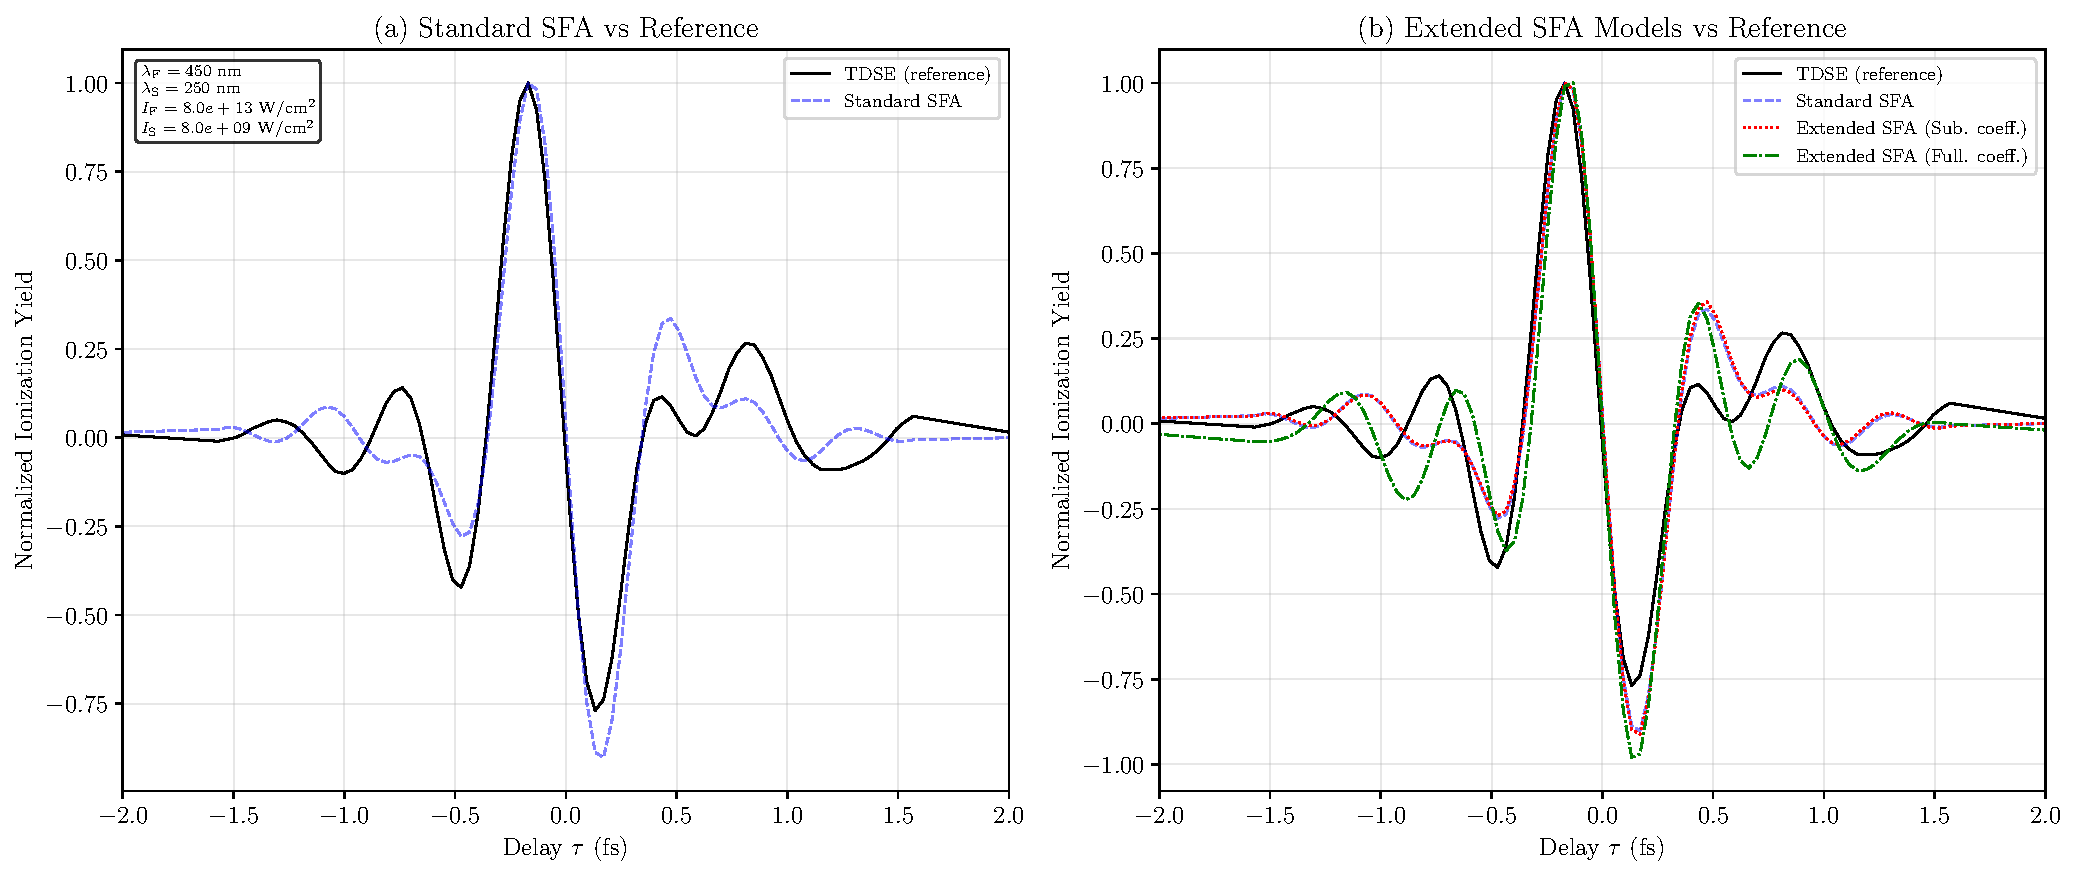
\includegraphics[width=1\textwidth]{../ionModel/python/plotsTIPTOE/2plot_SFA-comparison_1_BA.pdf}
    \caption[Comparison of SFA models and TDSE ionization yields]{Comparison of ionization yields from TIPTOE simulations between different SFA models and reference data from TDSE. 
            (a) Standart SFA overall does a good job reconstructing the ionization dynamics, but some parts it does not capture at all 
            (b) Comparison with extended SFA models with transitions to excited states neglected. }
    \label{fig:tiptoe_sfa_comparison}
\end{figure}


\bigskip
As mentioned in chapter 2, two major physical effects take place that are being carried over by the coefficient $c_0(t)$; the stark shift and the distortion of the ground state. 
By only using the phase of the $c_0(t)$, only the influence of the stark shift is taken into account.
That allows isolating different physical effects and their impact on ionization dynamics.

The figure \ref{fig:tiptoe_rate_stark}(a) shows exactly this approach, a TIPTOE scan but only with the phase of the coefficients:
\begin{equation*}
    c_n(t) = |c_n(t)|e^{i \phi_n(t)} \rightarrow c_n(t) = e^{i \phi_n(t)}
\end{equation*}
The results are obvious.
Almost all the contribution of the imporvement of ionization dynamics within the full hilbertspace coefficients are coming from the change in the energy levels.
This is strong evidence that the stark shift is indeed a very important effect in the ground state ionization dynamics.
The distortion of the ground state does not seem to have much impact.

Figure \ref{fig:tiptoe_rate_stark}(b) shows this in more detail.
In the rates, it is more obvious how much of an contribution the stark shift has in contrast to the distortion of the ground state.





\begin{figure}
    \centering
    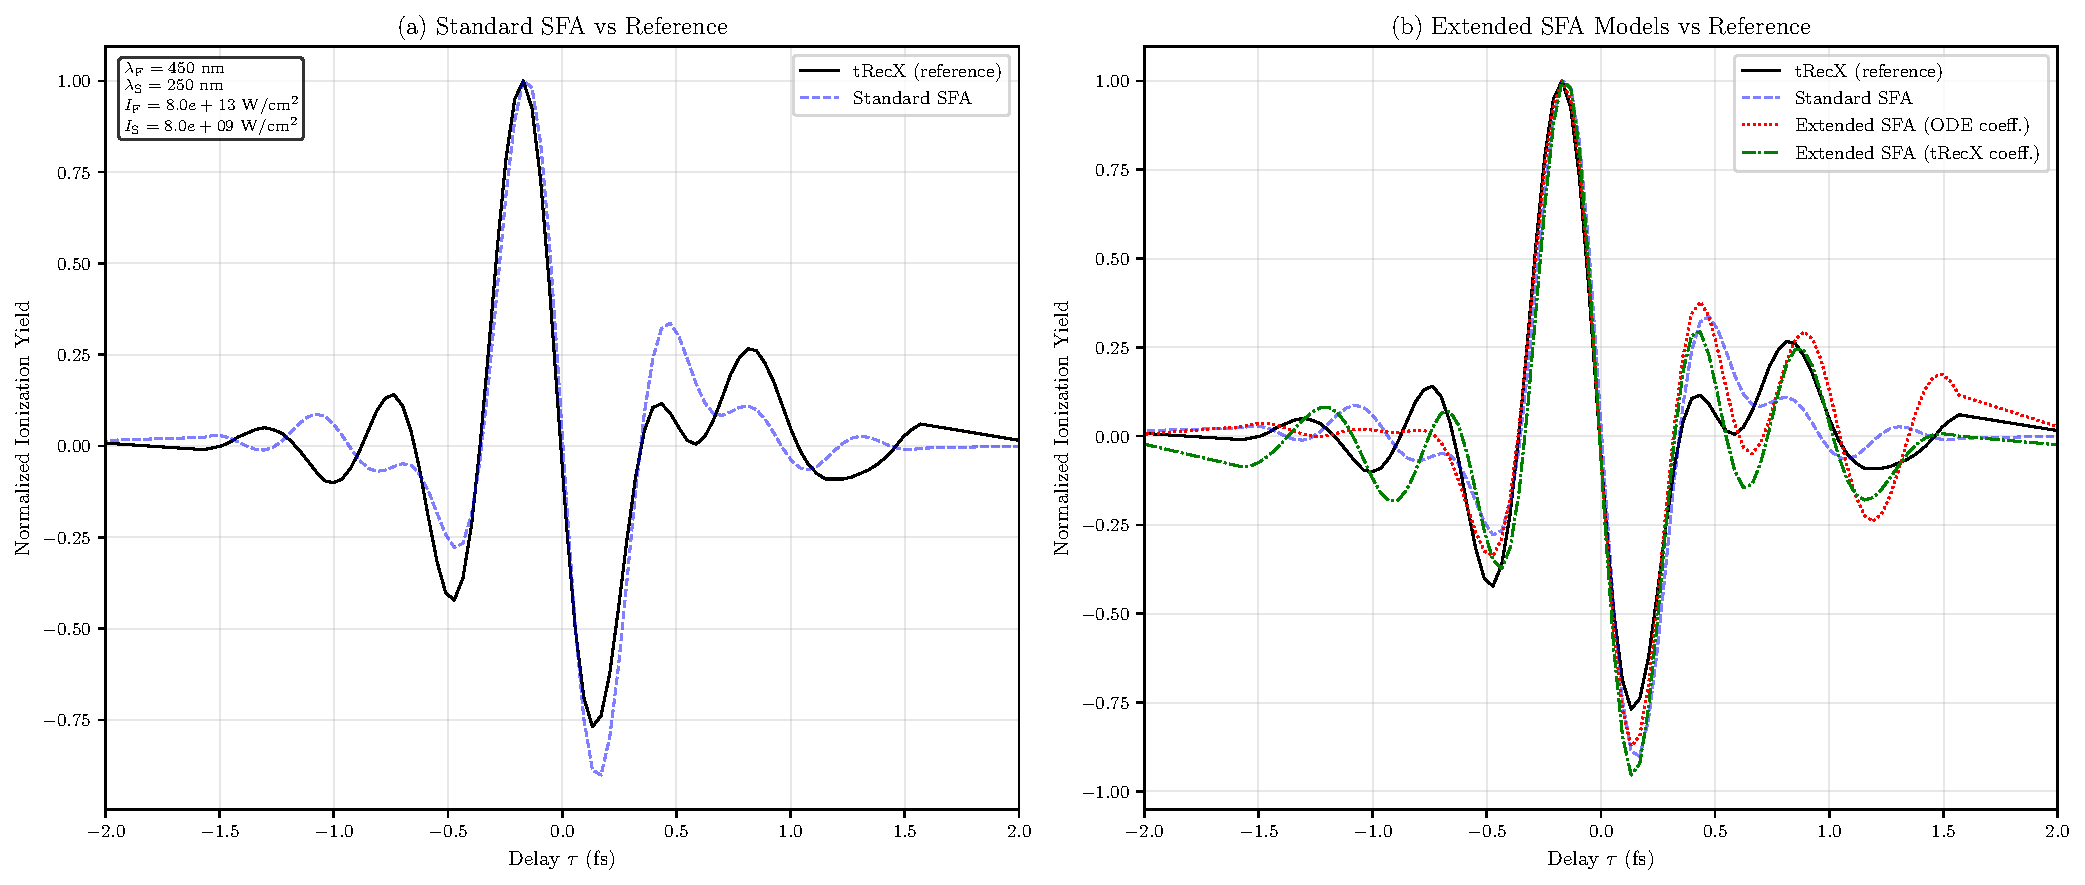
\includegraphics[width=1\textwidth]{../ionModel/python/plotsTIPTOE/2plot_SFA-comparison_2.pdf}
    \caption[Impact of stark effect on TIPTOE simulations and ionization rates]{Impact of stark shift on TIPTOE simulations and on ionization rates with transitions to excited states neglected. 
            (a) TIPTOE
            (b) Rate}
    \label{fig:tiptoe_rate_stark}
\end{figure}




\medskip
To make it in one sentence:
Taking only the stark effect of the ground state within the strong field approximation into account while determining the coefficients by solving the TDSE in the full hilbertspace, leads to a better reconstructing of the phase of the ionization dynamics in the offcycle region of the laser pulse than only considering the distortion of the ground state.



\paragraph{Difference in ionization yield between SFA and TDSE}
As mentioned in chapter 3, the Ionization yield in \ref{fig:tiptoe_sfa_comparison} is normalized, to see the actual difference better.
Further, because we are mostly interested in the dynamics and not the plain ionization yield, its normalized according to \eqref{eq:tiptoeprop_normalized}.
However, in the not normalized plot, one could see that the numerical solution of the TDSE is predicting a ionization probability orders of magnitude higher than the SFA model.
In addition to that, small changes in the in the delay of the signal pulse leads to bigger changes in the TDSE results than the SFA results, so the `reference' TIPTOE result is much more sensitive to changes in the laser field.
First observation can be interpreted by the fact that in SFA we are assuming, the electron sits in a continuum state after ionization so the elecotrn does not `feel' the coulomb potential anymore.
This is of course a very strong assumption, any much `harder' to achcieve for the electron. 
Imagine the laser has to really catapult the electron out of the atom to make this assumption approximately valid.
Therefore the overall ionization yield from the SFA model is much lower than the one from the TDSE.
Second, the numerical solution of the TDSE captures much more dynamics and physical effects of the ionization process.
Many different processes can happen during that time, and that could justify why the ionization yield of the TDSE is much more sensitive to changes in the elcetric field.

Both these observations are interesting, but can be expected from how the SFA model is constructed.
To make shure that the differences really do come from the `fundamentals' of the SFA model (i.e. the assumption that the final state is a continuum state), one has to make shure that is the only possible option for the differences.
The extended SFA model described in this thesis may give promising insights into this question.
During the research for this thesis, much work has gotten into the implementation of the extended SFA model, such that it incorparates also excited states .
Unfortunately, due to the limited time frame, I can not present certain results for this question. 
Latest TIPTOE results indicate that including excited states in the SFA rate help to a certain extend the difference in the order of magnitude between SFA and TDSE.
Also the cross-coupling terms in \eqref{eq:sfa_rate_improved} (i.e. $n_1 \neq n_2$) seems to have a significant contribution to the ionizatiion rate.
Furthermore, previous discussed results about the importance of the stark shift applies to excited states as well.
The shift in the energy level of the excited states playes a more significant role for the ionization rate than changes in the probability ampltidue of the coefficients.
The indicated changes in the order of magnitude of the ionization yield that could come from including excited states in the extended SFA model is could primarily coming from the dipole transition matrix elements.
For example this could be explained by the lase rpulse exciting the elctron to for isnatnce the 3p state and later ionizing it.
This will result in a much hgiher ionization probability overoll since more is possible.
However, this could not be shown here.
But these are not really results, only some hints.

















% On the left plot we see that tRecX is still orders of magnitude larger than the SFA results. 
% However, with excited states it goes in the right direction as can be seen on the right plot. 
% For three excited sates there is not much imporvement visible.
% Unfortunately, the results are no where close to the tRecX measurements. That indicates that there is some physics missing in the SFA model.
% If its not the excited states, the it must be something else.
% And because the change is so big it has to be something more fundamental.
% The first idea is that the interaction with the coulomb potential after ionization cannot be completely neglected, as it is done in the SFA model.
% Even though it is counterintuitive, becasue if the coulomb potential is still noticable for the electron after ionization, why would it increase the results we are seeing??????
% But this is in principle what our simulations are telling us. We can argue that we have two different ways of calculating the coefficients (ODE and tRecX) and the reproduce the same result.

% However it indicates that real ionization propabilities do have some characterisitcs that the improved SFA model does not capture.

% One also should make clear what the ODE coefficients do not capture. First, I implemented the code such that it ignores transitions not allowed by the dipole selection rules.

% So in principle, assuming my SFA modification was correct the TIPTOE results tell us that the coulomb potential is not negligible after all. 
% Maybe because the laser is not that intense (multiphoton ionization).
% But its difficult to test that because if I increase the laser intensity, the approximations I made with the coefficients is not valid anymore.

% Looking at not normalized results, tRecX is much more sensitive to the shift of probe and pump pulse, while excited SFA coefficients are not
% Maybe because tRecX takes into account all the dynamics and effects inside an atom, while excited SFA coefficients does not care that much.
% I would expect with tRecX coefficients more sensitive than with ODE coefficients???

% \section{Influence of Stark Shift and Polarisation}
% The Stark effect is the shift of the energy levels of an atom or molecule due to the presence of an external electric field.

% \begin{figure}[H]
%     \centering
%     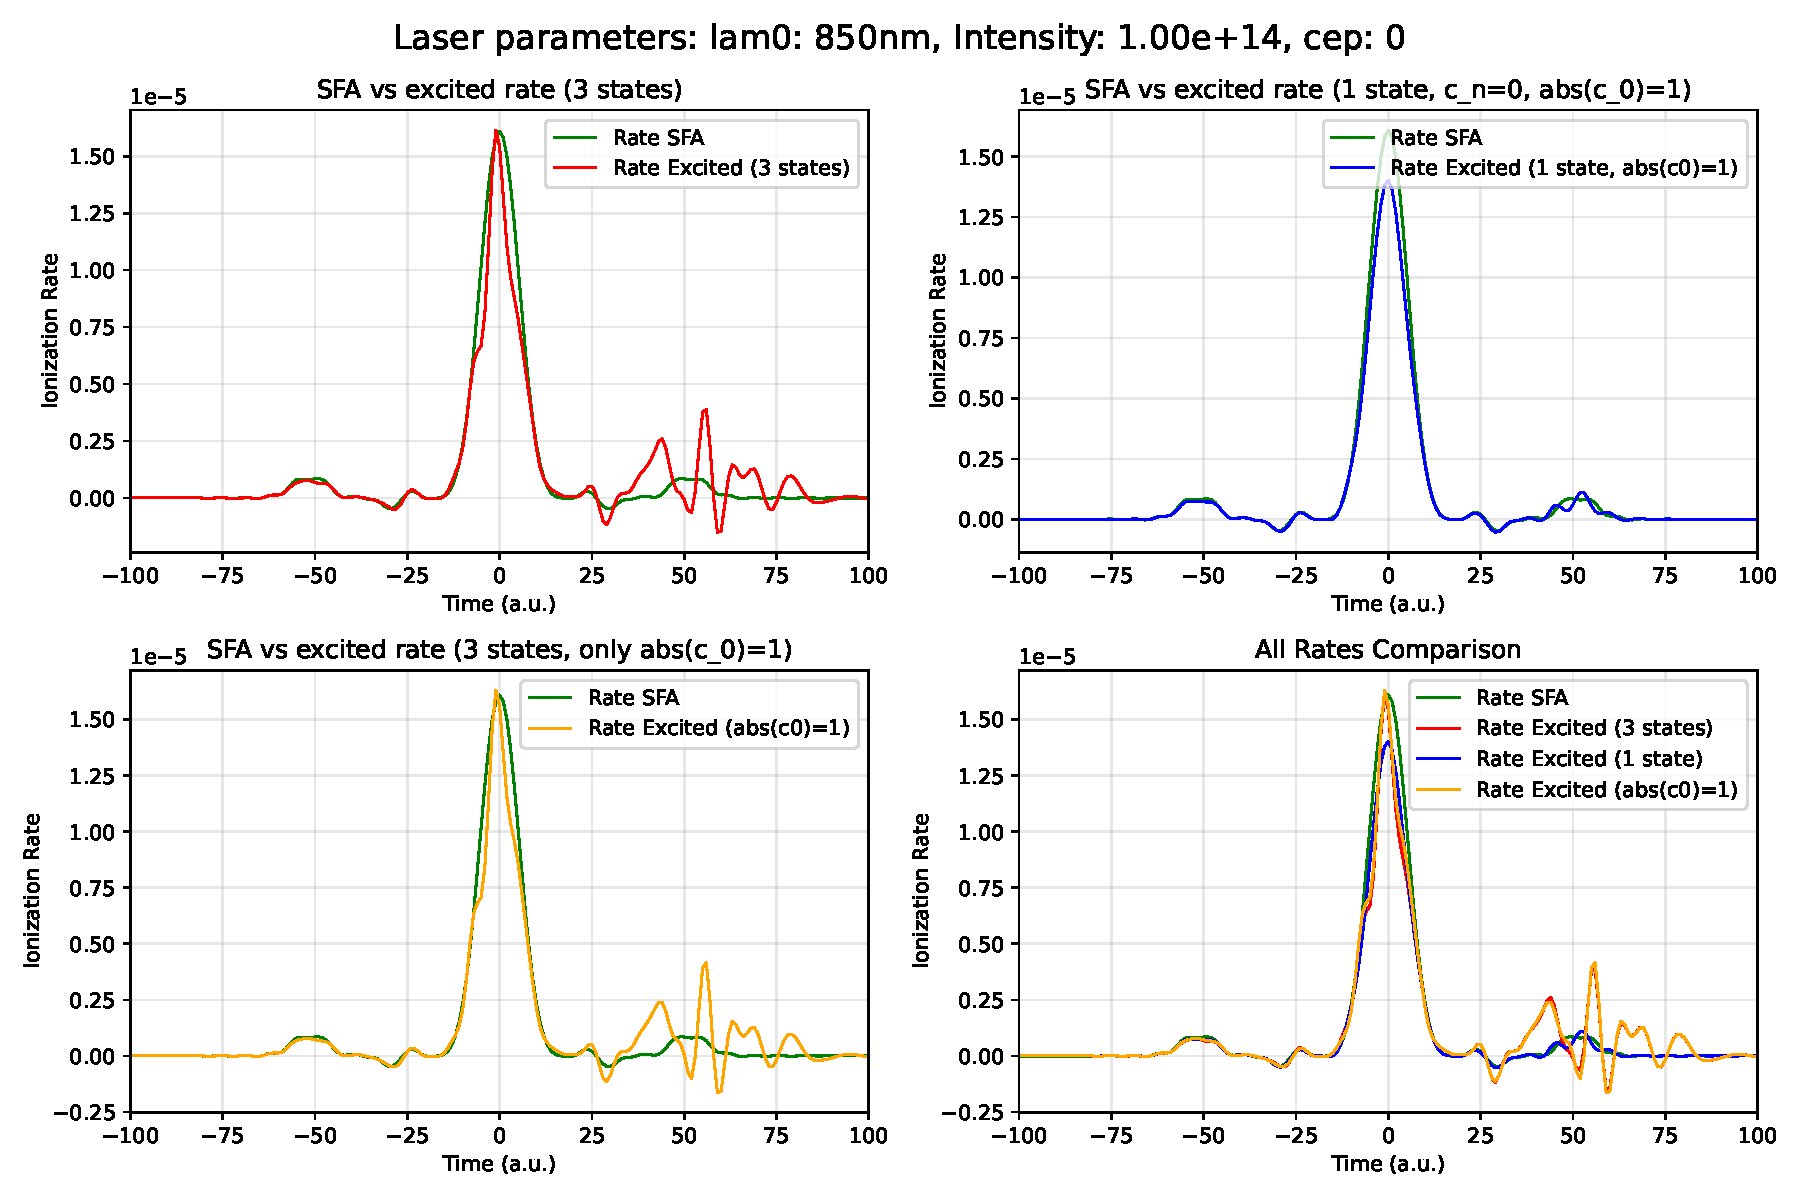
\includegraphics[width=0.9\textwidth]{figures/rate4_850_1.00e+14_onlystark.pdf}
%     \caption{stark effect}
%     \label{fig:starkeffect}
% \end{figure}

% Naiv: Stark effect changes energy in electron so its "harder" to ionise, thats why blue curve goes down (when excitedStates=1). 
% But thats not certainly the case because of stark effect, thats why only set absc0 to 1 and phase remains. 
% Example with oszillations with time dependent resonance frequency, and external force not at resonance but coincidence with oszillator resonance frequency so this may cause it.

% \bigskip
% Stark shift doesnt seem to have much contribution (sadly) but at least more than the polarisation of the ground state.

% Lets investigate the influence of first coefficient, nothing more. Only the phase has a contribution, the amplitude is not important.
% Thats because the amplitude determines something occupation propabilitiy, but the phase is $e^{-iEt}$ and if $E$ is shifted by a bit you can isolate it by just using purely the phase.\\
% Top right is the isolated stark effect








% \section{Laser Fields}
% Lorem ipsum dolor sit amet, consetetur sadipscing elitr, sed diam nonumy eirmod tempor invidunt ut labore et dolore magna aliquyam erat, sed diam voluptua. At vero eos et accusam et justo duo dolores et ea rebum. Stet clita kasd gubergren, no sea takimata sanctus est Lorem ipsum dolor sit amet. Lorem ipsum dolor sit amet, consetetur sadipscing elitr, sed diam nonumy eirmod tempor invidunt ut labore et dolore magna aliquyam erat, sed diam voluptua. At vero eos et accusam et justo duo dolores et ea rebum. Stet clita kasd gubergren, no sea takimata sanctus est Lorem ipsum dolor sit amet.


% \begin{equation}
%     \partial_t u = \mathcal{H}(t)  \lambda 
% \end{equation}

% \begin{figure}[H]
%     \centering
%     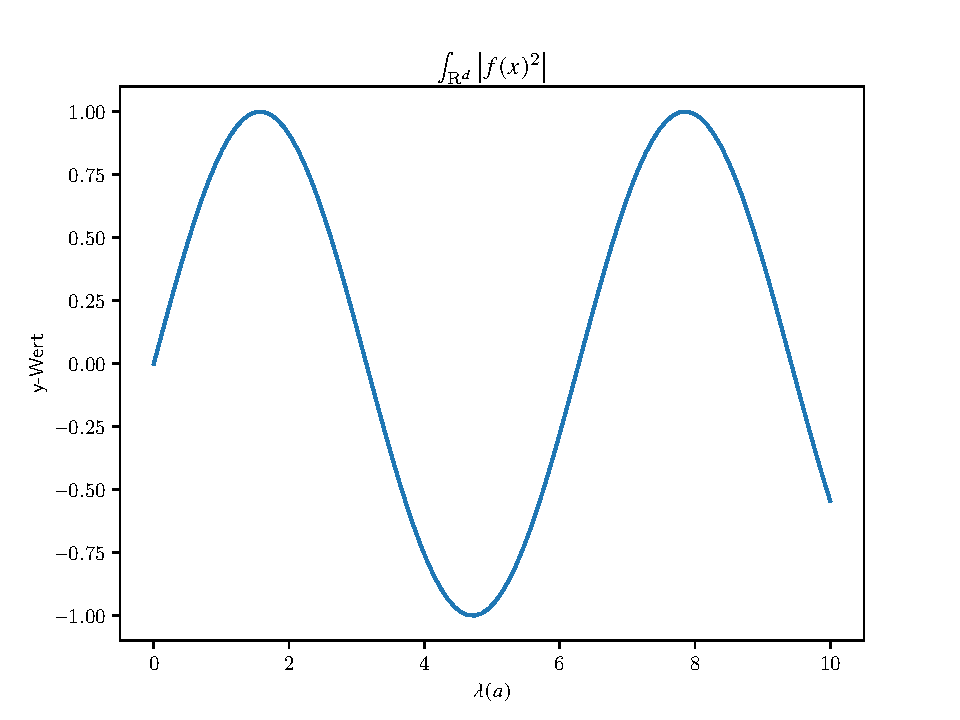
\includegraphics[width=0.5\textwidth]{figures/plot.pdf}
%     \caption{Sine function}
%     \label{fig:sinus}
% \end{figure}



% \begin{equation*}
%     \partial \A = \B
% \end{equation*}

% \medskip

% \begin{equation}
%     \int_{\R^d} \abs{f(x)}^2 \dd x = \int_{\R^d} \abs{\F f(\xi)}^2 \dd \xi
% \end{equation}

% \medskip

% \begin{equation}
%     %schrödinger equation
%     \ii \partial_t u = \mathcal{H}(t) \Ket{a} \lambda 
% \end{equation}

% \begin{equation}
%     \gimel \overrightarrow{a} \cos \mathrm{cos} \Rightarrow \Longrightarrow \nearrow 
% \end{equation}

\cleardoublepage


\chapter{Conclusion and Outlook}
% Could be good for GASFIR because GASFIR learns from exact SFA rate.\\
% What is more important, stark shift or else?\\

Lorem ipsum dolor sit amet, consetetur sadipscing elitr, sed diam nonumy eirmod tempor invidunt ut labore et dolore magna aliquyam erat, sed diam voluptua. At vero eos et accusam et justo duo dolores et ea rebum. Stet clita kasd gubergren, no sea takimata sanctus est Lorem ipsum dolor sit amet. Lorem ipsum dolor sit amet, consetetur sadipscing elitr, sed diam nonumy eirmod tempor invidunt ut labore et dolore magna aliquyam erat, sed diam voluptua. At vero eos et accusam et justo duo dolores et ea rebum. Stet clita kasd gubergren, no sea takimata sanctus est Lorem ipsum dolor sit amet.
\cleardoublepage


\appendix
\chapter{Volkov states}
Lorem ipsum dolor sit amet, consetetur sadipscing elitr, sed diam nonumy eirmod tempor invidunt ut labore et dolore magna aliquyam erat, sed diam voluptua. At vero eos et accusam et justo duo dolores et ea rebum. Stet clita kasd gubergren, no sea takimata sanctus est Lorem ipsum dolor sit amet. Lorem ipsum dolor sit amet, consetetur sadipscing elitr, sed diam nonumy eirmod tempor invidunt ut labore et dolore magna aliquyam erat, sed diam voluptua. At vero eos et accusam et justo duo dolores et ea rebum. Stet clita kasd gubergren, no sea takimata sanctus est Lorem ipsum dolor sit amet.
\cleardoublepage


\chapter{Dipole transition matrix elements}
% Solving TDSE for Hydrogen atom because it will be important later. also note the structure of wavefunction:
% \begin{equation*}
%     \psi_{nlm}(\uvec{x}) = \psi_{nlm}(r,\theta,\phi) = R_{nl}(r)Y_{lm}(\theta, \phi)
% \end{equation*}
% $E_n=\frac{Z^2}{2n^2}$
\label{sec:dipolematrixelements}
We want to derive the general transition dipole matrix elements into the continuum for an hydrogen-like atom. The general matrix element in our case is given by:
\begin{equation*}
    \uvec{d}(\uvec{p}) = \braket{\Pi|\vec{\hat{d}}|\Psi_{nlm}} \stackrel{\mathrm{a.u.}}{=} \braket{p|\vec{\hat{r}}|\Psi_{nlm}}
\end{equation*}
With $\ket{p}$ being a plane wave. By partitioning the $\hat{\vec{1}}$, and using the fact that $\vec{\hat{r}} \rightarrow i\nabla_{\uvec{p}}$ %Interesting because by choosing a certain way to display the operator we also choose a natural basis for the representation of the operator. Therefore I write \nabla_{\uvec{p}} instead of \nabla_{\vec{p}}.
in momentum representation we find a generel formula for the transition:
\begin{equation*}
    \uvec{d}(\uvec{p}) = i\nabla_{\uvec{p}}\int \dd^3\uvec{x}\,\psi_{nlm}(\uvec{x}) e^{-i\uvec{p}\cdot\uvec{x}} = i\nabla_{\uvec{p}}\phi_{nlm}(\uvec{p})
\end{equation*}
In principle, this integral or more precise the Fouriertransformation of the wavefunction is all we need to do.
Because of the structure of $\psi_{nlm}$ we can expect a result simular to (eqref psi=RY).
A posteriori we will see that:
\begin{equation*}
    \F\{\psi_{nlm}(\uvec{x})\} = \phi_{nlm}(\uvec{p}) = F_{nl}(p)Y_{lm}(\theta_p, \phi_p)
\end{equation*}
With $F_{nl}(p)$ being the Fouriertransform of the radial part of the wavefunction and $Y_{lm}(\theta_p, \phi_p)$ being the spherical harmonics in momentum space similar to the hydrogen atom in position space.




%%%%%%%%%%%%%%%%%%%%%%%
\subsection*{Momentum space}
We start with the so called plane wave expansion \cite{Jackson:1998nia} of the exponential part of the integral:
\begin{equation*}
    e^{i\uvec{p}\cdot\uvec{x}} = \sum_{l'=0}^\infty (2l'+1)i^{l'} j_{l'}(pr) P_{l'}(\uvec{p}\cdot\uvec{x}) = 4\pi\sum_{l'=0}^\infty \sum_{m'=-l'}^{l'} i^{l'} j_{l'}(pr) Y_{l'm'}(\theta_p, \phi_p) Y_{l'm'}^*(\theta_x, \phi_x)
\end{equation*}
With $j_l(pr)$ being the spherical bessel functions. Also note that we are integrating over spherical kordinates now. At first it looks messy but we can use the orthogonality of the spherical harmonics we can reduce the integral to:
\begin{equation*}
    \phi_{nlm}(\uvec{p}) = 4\pi \sum_{m=-l}^{l}Y_{lm}(\theta_p,\phi_p)i^l\underbrace{\int_{0}^{\infty}\dd r\,r^2j_l(pr)R_{nl}(r)}_{\tilde{R}_{nl}(p)}
\end{equation*}
This is the structure we were hoping for. Lets focus on the radial part $\tilde{R}_{nl}(p)$ of the integral.
The term $R_{nl}(r)$ represents the radial function of the hydrogen atom in position space and is independent of the magnetic bumber $m$. 
An exponential term dependent of $r$, a polynomial term dependent of $r$, the generalized Laguerre polynomials and the normalization constant. 
It would be convenient to have a closed expression for the generalzied Laguerre polynomials. 
I choose to represent them as following:
\begin{equation*}
    L_n^l(r) = \sum_{\iota=0}^{n} \frac{(-1)^{\iota}}{\iota!}\binom{n+l}{n-\iota}r^{\iota}
\end{equation*}
The Laguerre polynomials are therefore only dependent on and exponential term and finitely many polynomial terms. 
$\tilde{R}_{nl}(p)$ can be expressed (without prefactors and summation over $\iota$) as:
\begin{equation*}
    \int_{0}^{\infty}\dd r\,r^{2+l+\iota} e^{-\frac{Zr}{n}} j_l(pr)
\end{equation*}
Before we can solve the Integral using caomputational methods, we need to transform the spherical bessel function into the ordinary ones:
\begin{equation*}
    j_l(pr) = \sqrt{\frac{\pi}{2pr}}J_{l+\frac{1}{2}}(pr)
\end{equation*}
Now it is a good time to write all the prefactors and summations in one expression and look at the integral as a whole:
\begin{align*}
    \phi_{nlm}(\uvec{p}) =\ & \frac{\pi^{3/2}}{\sqrt{2p}}\sqrt{\left(\frac{2}{n}\right)^3\frac{(n-l-1)!}{n(n+1)!}}\\
    & \times \sum_{m=-l}^{l}\sum_{\iota=0}^{n-l-1}i^l\frac{(-1)^{\iota}}{\iota!}\left(\frac{2}{n}\right)^{l+\iota}\binom{n+l}{n-l-1}\underbrace{\int_{0}^{\infty}\dd r\,r^{l+\iota+\frac{3}{2}}e^{-\frac{Zr}{n}}J_{l+\frac{1}{2}}(pr)}_{(*)} Y_{lm}(\theta_p,\phi_p)
\end{align*}
To calculate the remaining Integral, I used mathematica, so I can not give a detailed explanation of that. Interestingly, there is an analytical solution for that. 
The result for $(*)$ is:
\begin{equation*}
    (*) = {}_2\tilde{F}_1\left(2 + l + \frac{\iota}{2}, \frac{1}{2}(5 + 2l + \iota); \frac{3}{2} + l; -\frac{n^2 p^2}{Z^2}\right)
\end{equation*}
With ${}_2\tilde{F}_1$ being the regularized hypergeometric function defined by:
\begin{equation*}
    {}_2\tilde{F}_1(a,b;c;z) = \frac{{}_2F_1(a,b;c;z)}{\Gamma(c)} = \frac{1}{\Gamma(a)\,\Gamma(b)} \sum_{n=0}^{\infty} \frac{\Gamma(a+n)\,\Gamma(b+n)}{\Gamma(c+n)} \frac{z^n}{n!}
\end{equation*}
The final formula $\phi_{nlm}(\uvec{p})$ that can be also found in [atoms and molekulse] in slightely different form, can then be expressed as:
\begin{align}
    \label{eq:phi_nlm}
    \phi_{nlm}(\uvec{p}) = \sum_{\iota=0}^{2l+1} \;
        & \frac{(-1)^{\iota} \; 2^{\iota + \frac{1}{2}} \; n \; (i n)^l \; (p^2)^{l/2} \; Z^{-l-3} \; \Gamma(2l+\iota+3)}{\iota!} \nonumber \\
        & \times \binom{l+n}{-l+n-\iota-1} 
        \sqrt{\frac{Z^3 \Gamma(n-l)}{\Gamma(l+n+1)}} \nonumber \\
        & \times Y_l^m(\theta_p, \phi_p) \,
        {}_2\tilde{F}_1\left(l+\frac{\iota}{2}+2, \frac{1}{2}(2l+\iota+3); l+\frac{3}{2}; -\frac{n^2 p^2}{Z^2}\right)
\end{align}








%%%%%%%%%%%%%%%%%%%%%%%
\subsection*{Transition Element}
Now all thats left is to differentiate \eqref{eq:phi_nlm} with respect to $\uvec{p}$. 


new eq
\begin{align}
    \sum _{\iota =0}^{2 l+1} \left(-\frac{(-1)^{\iota } n \text{Ip}^{-l-3} 2^{\iota -l-1} (i n)^l \left(p^2\right)^{l/2}
   \left(\frac{1}{\sqrt{p^2}}-\frac{\text{pz}^2}{\left(p^2\right)^{3/2}}\right) \Gamma (2 l+\iota +3) \binom{l+n}{-l+n-\iota -1} \sqrt{\frac{\text{Ip}^3 \Gamma
   (n-l)}{\Gamma (l+n+1)}} \, _2\tilde{F}_1\left(l+\frac{\iota }{2}+2,\frac{1}{2} (2 l+\iota +3);l+\frac{3}{2};-\frac{n^2 p^2}{4 \text{Ip}^2}\right) \left(\frac{m
   \text{pz} Y_l^m\left(\cos ^{-1}\left(\frac{\text{pz}}{\sqrt{p^2}}\right),\tan ^{-1}(\text{px},\text{py})\right)}{\sqrt{p^2}
   \sqrt{1-\frac{\text{pz}^2}{p^2}}}+\frac{\sqrt{\Gamma (l-m+1)} \sqrt{\Gamma (l+m+2)} e^{-i \tan ^{-1}(\text{px},\text{py})} Y_l^{m+1}\left(\cos
   ^{-1}\left(\frac{\text{pz}}{\sqrt{p^2}}\right),\tan ^{-1}(\text{px},\text{py})\right)}{\sqrt{\Gamma (l-m)} \sqrt{\Gamma (l+m+1)}}\right)}{\iota !
   \sqrt{1-\frac{\text{pz}^2}{p^2}}}+\frac{(-1)^{\iota } l n \text{pz} \text{Ip}^{-l-3} 2^{\iota -l-1} (i n)^l \left(p^2\right)^{\frac{l}{2}-1} \Gamma (2 l+\iota +3)
   \binom{l+n}{-l+n-\iota -1} \sqrt{\frac{\text{Ip}^3 \Gamma (n-l)}{\Gamma (l+n+1)}} \, _2\tilde{F}_1\left(l+\frac{\iota }{2}+2,\frac{1}{2} (2 l+\iota
   +3);l+\frac{3}{2};-\frac{n^2 p^2}{4 \text{Ip}^2}\right) Y_l^m\left(\cos ^{-1}\left(\frac{\text{pz}}{\sqrt{p^2}}\right),\tan
   ^{-1}(\text{px},\text{py})\right)}{\iota !}-\frac{(-1)^{\iota } n^3 \text{pz} \text{Ip}^{-l-5} 2^{\iota -l-3} \left(\frac{\iota }{2}+l+2\right) (\iota +2 l+3) (i
   n)^l \left(p^2\right)^{l/2} \Gamma (2 l+\iota +3) \binom{l+n}{-l+n-\iota -1} \sqrt{\frac{\text{Ip}^3 \Gamma (n-l)}{\Gamma (l+n+1)}} \,
   _2\tilde{F}_1\left(l+\frac{\iota }{2}+3,\frac{1}{2} (2 l+\iota +3)+1;l+\frac{5}{2};-\frac{n^2 p^2}{4 \text{Ip}^2}\right) Y_l^m\left(\cos
   ^{-1}\left(\frac{\text{pz}}{\sqrt{p^2}}\right),\tan ^{-1}(\text{px},\text{py})\right)}{\iota !}\right)
\end{align}
\begin{align}
    \sum_{\iota=0}^{2l+1} \Bigg(
        & -\frac{(-1)^{\iota} n\, \text{Ip}^{-l-3} 2^{\iota-l-1} (i n)^l (p^2)^{l/2}
        \left(\frac{1}{\sqrt{p^2}} - \frac{\text{pz}^2}{(p^2)^{3/2}}\right) \Gamma(2l+\iota+3)
        \binom{l+n}{-l+n-\iota-1}
        \sqrt{\frac{\text{Ip}^3 \Gamma(n-l)}{\Gamma(l+n+1)}} }{\iota! \sqrt{1-\frac{\text{pz}^2}{p^2}}} \nonumber \\
        & \times {}_2\tilde{F}_1\left(l+\frac{\iota}{2}+2, \frac{1}{2}(2l+\iota+3); l+\frac{3}{2}; -\frac{n^2 p^2}{4 \text{Ip}^2}\right)
        \left(
            \frac{m\, \text{pz}\, Y_l^m\left(\cos^{-1}\left(\frac{\text{pz}}{\sqrt{p^2}}\right), \tan^{-1}(\text{px},\text{py})\right)}
            {\sqrt{p^2} \sqrt{1-\frac{\text{pz}^2}{p^2}}}
        \right. \nonumber \\
        & \qquad \left.
            + \frac{
                \sqrt{\Gamma(l-m+1)} \sqrt{\Gamma(l+m+2)} e^{-i \tan^{-1}(\text{px},\text{py})}
                Y_l^{m+1}\left(\cos^{-1}\left(\frac{\text{pz}}{\sqrt{p^2}}\right), \tan^{-1}(\text{px},\text{py})\right)
            }{
                \sqrt{\Gamma(l-m)} \sqrt{\Gamma(l+m+1)}
            }
        \right) \nonumber \\
        & + \frac{(-1)^{\iota} l n\, \text{pz}\, \text{Ip}^{-l-3} 2^{\iota-l-1} (i n)^l (p^2)^{\frac{l}{2}-1}
            \Gamma(2l+\iota+3) \binom{l+n}{-l+n-\iota-1}
            \sqrt{\frac{\text{Ip}^3 \Gamma(n-l)}{\Gamma(l+n+1)}} }{\iota!}
        {}_2\tilde{F}_1\left(l+\frac{\iota}{2}+2, \frac{1}{2}(2l+\iota+3); l+\frac{3}{2}; -\frac{n^2 p^2}{4 \text{Ip}^2}\right)
        Y_l^m\left(\cos^{-1}\left(\frac{\text{pz}}{\sqrt{p^2}}\right), \tan^{-1}(\text{px},\text{py})\right) \nonumber \\
        & - \frac{(-1)^{\iota} n^3 \text{pz} \text{Ip}^{-l-5} 2^{\iota-l-3} \left(\frac{\iota}{2}+l+2\right) (\iota+2l+3) (i n)^l (p^2)^{l/2}
            \Gamma(2l+\iota+3) \binom{l+n}{-l+n-\iota-1}
            \sqrt{\frac{\text{Ip}^3 \Gamma(n-l)}{\Gamma(l+n+1)}} }{\iota!}
        {}_2\tilde{F}_1\left(l+\frac{\iota}{2}+3, \frac{1}{2}(2l+\iota+3)+1; l+\frac{5}{2}; -\frac{n^2 p^2}{4 \text{Ip}^2}\right)
        Y_l^m\left(\cos^{-1}\left(\frac{\text{pz}}{\sqrt{p^2}}\right), \tan^{-1}(\text{px},\text{py})\right)
    \Bigg)
\end{align}


% \phi_{nlm}(\uvec{p}) =\ & \sqrt{2} \left(\frac{1}{n}\right)^{-2 l-3} 
% \sqrt{\frac{(-l+n-1)!}{n^4 (l+n)!}} \\
% & \times \sum _{\iota =0}^{-l+n-1} 
% \frac{(-2)^{\iota } i^l p^l \Gamma (2 l+\iota +3)
% \binom{l+n}{-l+n-\iota -1} \, 
% {}_2\tilde{F}_1\left(l+\frac{\iota }{2}+2,\frac{1}{2} (2 l+\iota +3);l+\frac{3}{2};-n^2 p^2\right)}
% {\iota !} Y_{lm}(\theta_p,\phi_p)




% Some dipole matrix elements:\\
% First start with transforming the Schroedinger equation into momentum space %https://physics.stackexchange.com/questions/249400/schr%C3%B6dinger-equation-in-momentum-space
% Note that the prefactor does NOT depend on magentic quantumnumber m.\\
% Spherical harmonic: Instead of $Y_{lm}(\theta, \phi)$ you can write $Y_{lm}(\uvec{r})$ since $\uvec{r}=\hat{e}_x \sin(\theta)\cos(\phi)+\hat{e}_y\sin(\theta)\sin(\phi)+\hat{e}_z\cos(\theta)$\\
% The transition dipole matrix element is given by
% \begin{equation*}
%     % Analytical result for the integral
%     [ \int_0^\infty x^{\mu} e^{-\alpha x} J_\nu(\beta x) dx = \frac{\beta^\nu \Gamma(\mu+\nu+1)}{2^\nu \alpha^{\mu+\nu+1}} , {}_2F_1\left(\frac{\mu+\nu+1}{2}, \frac{\mu+\nu+2}{2}; \nu+1; -\frac{\beta^2}{\alpha^2}\right) ]
% \end{equation*}



























% \begin{equation*}
%     \vec{d}(\vec{p}) = \braket{\vec{p}|\vec{\hat{d}}|\Psi_{nlm}} = \nabla_{\vec{p}}\Psi_{nlm}(\vec{p})
% \end{equation*}
% \begin{equation*}
%     \braket{\vec{p}|100} = \frac{8 \sqrt{\pi }}{\sqrt{\frac{1}{a^3}} \left(a^2 p^2+1\right)^2}\text{if}\Re\left(\frac{1}{a}\right)>0
% \end{equation*}
% \begin{equation*}
%     \braket{\vec{p}|200} = \frac{32 \sqrt{2 \pi } \left(4 a^2 p^2-1\right)}{\sqrt{\frac{1}{a^3}} \left(4 a^2 p^2+1\right)^3}\text{if}\Re\left(\frac{1}{a}\right)>0
% \end{equation*}
% \begin{equation*}
%     \braket{\vec{p}|210} = -\frac{128 i \sqrt{2 \pi } \sqrt{\frac{1}{a^3}} a^4 p}{\left(4 a^2 p^2+1\right)^3}\text{if}\Re\left(\frac{1}{a}\right)>0
% \end{equation*}
% \begin{equation*}
%     \braket{\vec{p}|300} = \frac{72 \sqrt{3 \pi } \left(81 a^4 p^4-30 a^2 p^2+1\right)}{\sqrt{\frac{1}{a^3}} \left(9 a^2p^2+1\right)^4}\text{ if }\Re\left(\frac{1}{a}\right)>0
% \end{equation*}
% \begin{equation*}
%     \braket{\vec{p}|310} = -\frac{864 i \sqrt{2 \pi } \sqrt{\frac{1}{a^3}} a^4 p \left(9 a^2 p^2-1\right)}{\left(9 a^2 p^2+1\right)^4}
% \end{equation*}
% \begin{equation*}
%     \braket{\vec{p}|320} = -\frac{1728 \sqrt{6 \pi } \sqrt{\frac{1}{a^3}} a^5 p^2}{\left(9 a^2 p^2+1\right)^4}
% \end{equation*}
% \begin{equation*}
%     \braket{\vec{p}|400} = \frac{256 \sqrt{\pi } \left(4096 a^6 p^6-1792 a^4 p^4+112 a^2 p^2-1\right)}{\sqrt{\frac{1}{a^3}}\left(16 a^2 p^2+1\right)^5}\text{ if }\Re\left(\frac{1}{a}\right)>0
% \end{equation*}
% \begin{equation*}
%     \braket{\vec{p}|410} = -\frac{2048 i \sqrt{\frac{\pi }{5}} \left(\frac{1}{a^3}\right)^{3/2} a^7 p \left(32 a^2 p^2 \left(40 a^2p^2-7\right)+5\right)}{\left(16 a^2 p^2+1\right)^5}\text{ if }\Re\left(\frac{1}{a}\right)>0
% \end{equation*}
% \begin{equation*}
%     \braket{\vec{p}|420} = -\frac{32768 \sqrt{\pi } \sqrt{\frac{1}{a^3}} a^5 p^2 \left(16 a^2 p^2-1\right)}{\left(16 a^2 p^2+1\right)^5}
% \end{equation*}
% \begin{equation*}
%     \braket{\vec{p}|430} = \frac{262144 i \sqrt{\frac{\pi }{5}} \sqrt{\frac{1}{a^3}} a^6 p^3}{\left(16 a^2 p^2+1\right)^5}
% \end{equation*}
% \begin{equation*}
%     \braket{\vec{p}|900} = \frac{1944 \sqrt{\pi } \left(27 a^2 p^2-1\right) \left(243 a^2 p^2-1\right) \left(243 a^2 p^2 \left(6561
%     a^4 p^4-729 a^2 p^2+11\right)-1\right) \left(729 \left(243 a^6 p^6-99 a^4 p^4+a^2
%     p^2\right)-1\right)}{\sqrt{\frac{1}{a^3}} \left(81 a^2 p^2+1\right)^{10}}\text{ if
%     }\Re\left(\frac{1}{a}\right)>0
% \end{equation*}
% \begin{equation*}
%     \braket{\vec{p}|510} = -\frac{4000 i \sqrt{10 \pi } \sqrt{\frac{1}{a^3}} a^4 p \left(15625 a^6 p^6-3375 a^4 p^4+135 a^2
%     p^2-1\right)}{\left(25 a^2 p^2+1\right)^6}\text{ if }\Re\left(\frac{1}{a}\right)>0
% \end{equation*}
\cleardoublepage


% \chapter{Semi-classical Hamiltonian}
% \label{sec:semiclassichamilton}
Here we will derive semi classical Hamiltonian. This part mainly follows \cite{LandauLifschitzBand2}.
\begin{equation}
    \hat{\Hs}(\uvec{x}, t) = \frac{1}{2m}(\vec{\hat{P}} - e \vec{A}(\uvec{x}, t))^2 + e \varphi(\uvec{x}, t)
\end{equation}
% \cleardoublepage


% \chapter{TDSE Solution}
% \begin{lstlisting}[language=Python]
    import numpy as np
    
    print("hello")
    \end{lstlisting}
    testa
    \begin{lstlisting}[language=C++]
    #include <iostream>
    
    int main() {
        std::cout << "Hello, World!" << std::endl;
        return 0;
    }
    \end{lstlisting}
    
    
% \cleardoublepage


\chapter{Code}
\begin{lstlisting}[language=Python]
    for state in range(excitedStates):
        for stateRange in range(excitedStates):
            cLeft = coefficients[state, :]
            cRight = coefficients[stateRange, :]
            f0 = np.zeros((Tar.size, tar.size), dtype=np.cdouble)
            phase0 = np.zeros((Tar.size, tar.size), dtype=np.cdouble)
            for i in prange(Tar.size):
                Ti=Ti_ar[i]
                for j in range(tar.size):
                    tj=N+nmin+j*n
                    tp=tj+Ti
                    tm=tj-Ti
                    if tp>=0 and tp<EF.size and tm>=0 and tm<EF.size:
                        VPt = 0 # VP[tj]
                        T= Ti*dT
                        DelA = (intA[tp] - intA[tm])-2*VPt*T
                        VP_p=VP[tp]-VPt
                        VP_m=VP[tm]-VPt
                        counter += 1
                        #print("counter", counter)         #first state and normal SFA are exactly 4pi apart 
                        nL, lL, mL = config[state]
                        nR, lR, mR = config[stateRange]
                        f_t_1= np.conjugate(transitionElementtest(nL, lL, mL, p, pz, VP_m, E_g))*transitionElementtest(nR, lR, mR, p, pz, VP_p, E_g)
                        #f_t_1= (pz+VP_p)/(p**2+VP_p**2+2*pz*VP_p+2*E_g)**3*(pz+VP_m)/(p**2+VP_m**2+2*pz*VP_m+2*E_g)**3
                        G1_T_p=np.trapz(f_t_1*np.exp(1j*pz*DelA)*np.sin(theta), Theta_grid)
                        G1_T=np.trapz(G1_T_p*window*p_grid**2*np.exp(1j*p_grid**2*T), p_grid)
                        DelA = DelA + 2 * VPt * T
                        phase0[i, j]  = (intA2[tp] - intA2[tm])/2  + T*VPt**2-VPt*DelA + eigenEnergy[state]*tm - eigenEnergy[stateRange]*tp 
                        f0[i, j] = EF[tp]*EF[tm]*G1_T*np.conjugate(cLeft[tm])*cRight[tp]#(np.real(c[tp])*np.real(c[tm])+np.imag(c[tp])*np.imag(c[tm]))
            print("state", state, "stateRange", stateRange)
            print("config", config[state], "configRange", config[stateRange])
            plt.plot(tar, 2*np.real(IOF(Tar, f0, (phase0)*1j)))
            plt.show()
            plt.close()
            rate += 2*np.real(IOF(Tar, f0, (phase0)*1j))    #*c[np.newaxis, :]
    return rate
    \end{lstlisting}
    testa
    \begin{lstlisting}[language=C++]
    #include <iostream>
    
    int main() {
        std::cout << "Hello, World!" << std::endl;
        return 0;
    }
\end{lstlisting}
    
\cleardoublepage


\phantomsection % ...
\addcontentsline{toc}{chapter}{Bibliography} % ...
\bibliographystyle{plain}
\bibliography{bibliography}
\cleardoublepage


\chapter*{Declaration of Authorship}
\addcontentsline{toc}{chapter}{Declaration of Authorship}
\emph{Hiermit erkläre ich, die vorliegende Arbeit selbständig verfasst zu haben und keine anderen als die in der Arbeit angegebenen Quellen und Hilfsmittel benutzt zu haben.}

\vspace{2cm}  
\noindent
\begin{tabular}{p{7cm} p{7cm}}
    München, den 20.6.2025 & \rule{6cm}{0.4pt} \\  
    & Unterschrift
\end{tabular}


\end{document}

%-----------------------------------------------------------------